% Options for packages loaded elsewhere
% Options for packages loaded elsewhere
\PassOptionsToPackage{unicode}{hyperref}
\PassOptionsToPackage{hyphens}{url}
\PassOptionsToPackage{dvipsnames,svgnames,x11names}{xcolor}
%
\documentclass[
  letterpaper,
  DIV=11,
  numbers=noendperiod]{scrartcl}
\usepackage{xcolor}
\usepackage{amsmath,amssymb}
\setcounter{secnumdepth}{-\maxdimen} % remove section numbering
\usepackage{iftex}
\ifPDFTeX
  \usepackage[T1]{fontenc}
  \usepackage[utf8]{inputenc}
  \usepackage{textcomp} % provide euro and other symbols
\else % if luatex or xetex
  \usepackage{unicode-math} % this also loads fontspec
  \defaultfontfeatures{Scale=MatchLowercase}
  \defaultfontfeatures[\rmfamily]{Ligatures=TeX,Scale=1}
\fi
\usepackage{lmodern}
\ifPDFTeX\else
  % xetex/luatex font selection
\fi
% Use upquote if available, for straight quotes in verbatim environments
\IfFileExists{upquote.sty}{\usepackage{upquote}}{}
\IfFileExists{microtype.sty}{% use microtype if available
  \usepackage[]{microtype}
  \UseMicrotypeSet[protrusion]{basicmath} % disable protrusion for tt fonts
}{}
\makeatletter
\@ifundefined{KOMAClassName}{% if non-KOMA class
  \IfFileExists{parskip.sty}{%
    \usepackage{parskip}
  }{% else
    \setlength{\parindent}{0pt}
    \setlength{\parskip}{6pt plus 2pt minus 1pt}}
}{% if KOMA class
  \KOMAoptions{parskip=half}}
\makeatother
% Make \paragraph and \subparagraph free-standing
\makeatletter
\ifx\paragraph\undefined\else
  \let\oldparagraph\paragraph
  \renewcommand{\paragraph}{
    \@ifstar
      \xxxParagraphStar
      \xxxParagraphNoStar
  }
  \newcommand{\xxxParagraphStar}[1]{\oldparagraph*{#1}\mbox{}}
  \newcommand{\xxxParagraphNoStar}[1]{\oldparagraph{#1}\mbox{}}
\fi
\ifx\subparagraph\undefined\else
  \let\oldsubparagraph\subparagraph
  \renewcommand{\subparagraph}{
    \@ifstar
      \xxxSubParagraphStar
      \xxxSubParagraphNoStar
  }
  \newcommand{\xxxSubParagraphStar}[1]{\oldsubparagraph*{#1}\mbox{}}
  \newcommand{\xxxSubParagraphNoStar}[1]{\oldsubparagraph{#1}\mbox{}}
\fi
\makeatother

\usepackage{color}
\usepackage{fancyvrb}
\newcommand{\VerbBar}{|}
\newcommand{\VERB}{\Verb[commandchars=\\\{\}]}
\DefineVerbatimEnvironment{Highlighting}{Verbatim}{commandchars=\\\{\}}
% Add ',fontsize=\small' for more characters per line
\usepackage{framed}
\definecolor{shadecolor}{RGB}{241,243,245}
\newenvironment{Shaded}{\begin{snugshade}}{\end{snugshade}}
\newcommand{\AlertTok}[1]{\textcolor[rgb]{0.68,0.00,0.00}{#1}}
\newcommand{\AnnotationTok}[1]{\textcolor[rgb]{0.37,0.37,0.37}{#1}}
\newcommand{\AttributeTok}[1]{\textcolor[rgb]{0.40,0.45,0.13}{#1}}
\newcommand{\BaseNTok}[1]{\textcolor[rgb]{0.68,0.00,0.00}{#1}}
\newcommand{\BuiltInTok}[1]{\textcolor[rgb]{0.00,0.23,0.31}{#1}}
\newcommand{\CharTok}[1]{\textcolor[rgb]{0.13,0.47,0.30}{#1}}
\newcommand{\CommentTok}[1]{\textcolor[rgb]{0.37,0.37,0.37}{#1}}
\newcommand{\CommentVarTok}[1]{\textcolor[rgb]{0.37,0.37,0.37}{\textit{#1}}}
\newcommand{\ConstantTok}[1]{\textcolor[rgb]{0.56,0.35,0.01}{#1}}
\newcommand{\ControlFlowTok}[1]{\textcolor[rgb]{0.00,0.23,0.31}{\textbf{#1}}}
\newcommand{\DataTypeTok}[1]{\textcolor[rgb]{0.68,0.00,0.00}{#1}}
\newcommand{\DecValTok}[1]{\textcolor[rgb]{0.68,0.00,0.00}{#1}}
\newcommand{\DocumentationTok}[1]{\textcolor[rgb]{0.37,0.37,0.37}{\textit{#1}}}
\newcommand{\ErrorTok}[1]{\textcolor[rgb]{0.68,0.00,0.00}{#1}}
\newcommand{\ExtensionTok}[1]{\textcolor[rgb]{0.00,0.23,0.31}{#1}}
\newcommand{\FloatTok}[1]{\textcolor[rgb]{0.68,0.00,0.00}{#1}}
\newcommand{\FunctionTok}[1]{\textcolor[rgb]{0.28,0.35,0.67}{#1}}
\newcommand{\ImportTok}[1]{\textcolor[rgb]{0.00,0.46,0.62}{#1}}
\newcommand{\InformationTok}[1]{\textcolor[rgb]{0.37,0.37,0.37}{#1}}
\newcommand{\KeywordTok}[1]{\textcolor[rgb]{0.00,0.23,0.31}{\textbf{#1}}}
\newcommand{\NormalTok}[1]{\textcolor[rgb]{0.00,0.23,0.31}{#1}}
\newcommand{\OperatorTok}[1]{\textcolor[rgb]{0.37,0.37,0.37}{#1}}
\newcommand{\OtherTok}[1]{\textcolor[rgb]{0.00,0.23,0.31}{#1}}
\newcommand{\PreprocessorTok}[1]{\textcolor[rgb]{0.68,0.00,0.00}{#1}}
\newcommand{\RegionMarkerTok}[1]{\textcolor[rgb]{0.00,0.23,0.31}{#1}}
\newcommand{\SpecialCharTok}[1]{\textcolor[rgb]{0.37,0.37,0.37}{#1}}
\newcommand{\SpecialStringTok}[1]{\textcolor[rgb]{0.13,0.47,0.30}{#1}}
\newcommand{\StringTok}[1]{\textcolor[rgb]{0.13,0.47,0.30}{#1}}
\newcommand{\VariableTok}[1]{\textcolor[rgb]{0.07,0.07,0.07}{#1}}
\newcommand{\VerbatimStringTok}[1]{\textcolor[rgb]{0.13,0.47,0.30}{#1}}
\newcommand{\WarningTok}[1]{\textcolor[rgb]{0.37,0.37,0.37}{\textit{#1}}}

\usepackage{longtable,booktabs,array}
\usepackage{calc} % for calculating minipage widths
% Correct order of tables after \paragraph or \subparagraph
\usepackage{etoolbox}
\makeatletter
\patchcmd\longtable{\par}{\if@noskipsec\mbox{}\fi\par}{}{}
\makeatother
% Allow footnotes in longtable head/foot
\IfFileExists{footnotehyper.sty}{\usepackage{footnotehyper}}{\usepackage{footnote}}
\makesavenoteenv{longtable}
\usepackage{graphicx}
\makeatletter
\newsavebox\pandoc@box
\newcommand*\pandocbounded[1]{% scales image to fit in text height/width
  \sbox\pandoc@box{#1}%
  \Gscale@div\@tempa{\textheight}{\dimexpr\ht\pandoc@box+\dp\pandoc@box\relax}%
  \Gscale@div\@tempb{\linewidth}{\wd\pandoc@box}%
  \ifdim\@tempb\p@<\@tempa\p@\let\@tempa\@tempb\fi% select the smaller of both
  \ifdim\@tempa\p@<\p@\scalebox{\@tempa}{\usebox\pandoc@box}%
  \else\usebox{\pandoc@box}%
  \fi%
}
% Set default figure placement to htbp
\def\fps@figure{htbp}
\makeatother





\setlength{\emergencystretch}{3em} % prevent overfull lines

\providecommand{\tightlist}{%
  \setlength{\itemsep}{0pt}\setlength{\parskip}{0pt}}



 


\usepackage{booktabs}
\usepackage{longtable}
\usepackage{array}
\usepackage{multirow}
\usepackage{wrapfig}
\usepackage{float}
\usepackage{colortbl}
\usepackage{pdflscape}
\usepackage{tabu}
\usepackage{threeparttable}
\usepackage{threeparttablex}
\usepackage[normalem]{ulem}
\usepackage{makecell}
\usepackage{xcolor}
\usepackage{fvextra}
\usepackage{longtable}
\usepackage{booktabs}
\DefineVerbatimEnvironment{Highlighting}{Verbatim}{breaklines,commandchars=\\\{\}}
\DefineVerbatimEnvironment{OutputCode}{Verbatim}{breaklines,commandchars=\\\{\}}
\KOMAoption{captions}{tableheading}
\makeatletter
\@ifpackageloaded{caption}{}{\usepackage{caption}}
\AtBeginDocument{%
\ifdefined\contentsname
  \renewcommand*\contentsname{Table of contents}
\else
  \newcommand\contentsname{Table of contents}
\fi
\ifdefined\listfigurename
  \renewcommand*\listfigurename{List of Figures}
\else
  \newcommand\listfigurename{List of Figures}
\fi
\ifdefined\listtablename
  \renewcommand*\listtablename{List of Tables}
\else
  \newcommand\listtablename{List of Tables}
\fi
\ifdefined\figurename
  \renewcommand*\figurename{Figure}
\else
  \newcommand\figurename{Figure}
\fi
\ifdefined\tablename
  \renewcommand*\tablename{Table}
\else
  \newcommand\tablename{Table}
\fi
}
\@ifpackageloaded{float}{}{\usepackage{float}}
\floatstyle{ruled}
\@ifundefined{c@chapter}{\newfloat{codelisting}{h}{lop}}{\newfloat{codelisting}{h}{lop}[chapter]}
\floatname{codelisting}{Listing}
\newcommand*\listoflistings{\listof{codelisting}{List of Listings}}
\makeatother
\makeatletter
\makeatother
\makeatletter
\@ifpackageloaded{caption}{}{\usepackage{caption}}
\@ifpackageloaded{subcaption}{}{\usepackage{subcaption}}
\makeatother
\usepackage{bookmark}
\IfFileExists{xurl.sty}{\usepackage{xurl}}{} % add URL line breaks if available
\urlstyle{same}
\hypersetup{
  pdftitle={Problem Set 4 revised},
  pdfauthor={Abhishu Karki},
  colorlinks=true,
  linkcolor={blue},
  filecolor={Maroon},
  citecolor={Blue},
  urlcolor={Blue},
  pdfcreator={LaTeX via pandoc}}


\title{Problem Set 4 revised}
\author{Abhishu Karki}
\date{}
\begin{document}
\maketitle


\section{LPG dependence in Nepali Households as Recorded in 2021 Nepal
Census.}\label{lpg-dependence-in-nepali-households-as-recorded-in-2021-nepal-census.}

\subsection{Summary}\label{summary}

This report analyzes household cooking fuel use in Nepal using data from
the 2021 National Population and Housing Census, with the intention of
understanding the role of liquefied petroleum gas (LPG). This analysis
shows that LPG has become the main cooking fuel in cities and towns,
while wood remains dominant in rural areas. This pattern matters because
Nepal imports all of its LPG and is therefore exposed to global supply
disruptions. Recent instability around the Strait of Hormuz has
contributed to shortages and price hikes that Nepali households are
currently experiencing. By examining cooking fuel use across provinces,
districts, and types of local governments, this report shows that
dependence on LPG is highly uneven within Nepal. Urban areas benefit
most from LPG, so they are also the most vulnerable when imports are
disrupted.The findings highlight an important trade‑off between cleaner
cooking and energy security in a net importer country like Nepal.

\subsection{Motivation}\label{motivation}

Over the past decade, Nepal has made progress in moving households away
from traditional cooking fuels such as firewood, biogas, cow dung etc.
and LPG has played a central role in this transition. However, Nepal
does not produce LPG domestically and relies entirely on imports, mostly
through regional supply chains connected to global energy markets. This
dependence has cost household a large price along many crisis that the
Nepali economy has faced, like the 2015 earthquake, India's economic
blockage, Covid etc.; And now is even more visible during recent
shortages and price increases linked to geopolitical tensions affecting
the Strait of Hormuz. When supply routes are disrupted, Nepali
households feel the effects almost immediately. Understanding how
widespread LPG use is and where it is most concentrated, is important
for energy planning and policy. National averages alone do not show
which regions are most exposed to LPG shortages or which areas are less
affected because they still rely on domestic fuels. This report aims to
fill that gap by using detailed census data to map cooking fuel use
across Nepal and assess the country's vulnerability to LPG supply
shocks.

\subsection{Data and Measurement}\label{data-and-measurement}

The analysis uses data from Nepal's 2021 National Population and Housing
Census, retrieved from
\href{https://censusnepal.cbs.gov.np/results/population}{Government of
Nepal, National Statistics Office}, which reports the number of
households using different fuels for cooking. The fuels included in the
dataset are Wood, LPG, Electricity, Bio gas, Cow dung, Kerosene, and
Other sources. For visualization purpose, all sources except for the two
big ones i.e.~Wood and LPG, have been consolidated as `Other sources'.
The data are available at multiple levels, including province, district,
and local government.

Local governments are grouped into four types, from most to least urban:

\begin{enumerate}
\def\labelenumi{\arabic{enumi}.}
\tightlist
\item
  Metropolitan City
\item
  Sub‑Metropolitan City
\item
  Municipality
\item
  Gaunpalika (rural municipalities)
\end{enumerate}

\begingroup\fontsize{8}{10}\selectfont

\begin{longtable}[t]{>{}lcccc}

\caption{\label{tbl-percentlocook}Percentage Distribution of Cooking
Fuel by Local Level Type}

\tabularnewline

\\
\toprule
\cellcolor[HTML]{2E86AB}{\textcolor[HTML]{F2F0EF}{\textbf{Local\_type}}} & \cellcolor[HTML]{2E86AB}{\textcolor[HTML]{F2F0EF}{\textbf{National\_Share}}} & \cellcolor[HTML]{2E86AB}{\textcolor[HTML]{F2F0EF}{\textbf{Wood}}} & \cellcolor[HTML]{2E86AB}{\textcolor[HTML]{F2F0EF}{\textbf{LPG}}} & \cellcolor[HTML]{2E86AB}{\textcolor[HTML]{F2F0EF}{\textbf{Others}}}\\
\midrule
\endfirsthead
\caption[]{Percentage Distribution of Cooking Fuel by Local Level Type \textit{(continued)}}\\
\toprule
\cellcolor[HTML]{2E86AB}{\textcolor[HTML]{F2F0EF}{\textbf{Local\_type}}} & \cellcolor[HTML]{2E86AB}{\textcolor[HTML]{F2F0EF}{\textbf{National\_Share}}} & \cellcolor[HTML]{2E86AB}{\textcolor[HTML]{F2F0EF}{\textbf{Wood}}} & \cellcolor[HTML]{2E86AB}{\textcolor[HTML]{F2F0EF}{\textbf{LPG}}} & \cellcolor[HTML]{2E86AB}{\textcolor[HTML]{F2F0EF}{\textbf{Others}}}\\
\midrule
\endhead

\endfoot
\bottomrule
\endlastfoot
\cellcolor[HTML]{F2F0EF}{\textcolor[HTML]{2E86AB}{\textbf{Metropolitian City}}} & 9.9\% & 7\% & 91.6\% & 1.5\%\\
\cmidrule{1-5}\pagebreak[0]
\cellcolor[HTML]{F2F0EF}{\textcolor[HTML]{2E86AB}{\textbf{Sub-Metropolitian City}}} & 6.8\% & 26.4\% & 71.1\% & 2.5\%\\
\cmidrule{1-5}\pagebreak[0]
\cellcolor[HTML]{F2F0EF}{\textcolor[HTML]{2E86AB}{\textbf{Municipality}}} & 50.5\% & 47.4\% & 47.9\% & 4.7\%\\
\cmidrule{1-5}\pagebreak[0]
\cellcolor[HTML]{F2F0EF}{\textcolor[HTML]{2E86AB}{\textbf{Gaunpalika}}} & 32.8\% & 75\% & 18.9\% & 6.1\%\\*
\multicolumn{5}{l}{\rule{0pt}{1em}Source: Census 2021.}\\

\end{longtable}

\endgroup{}

Nepal is politically divided into 7 states, that span cross 77 districts
and account for 753 local levels. The four local level division are
based on population size, urban/rural character, and administrative
needs.

Table~\ref{tbl-percentlocook} quantifies the distribution of cooking
fuel use across these local government types. It shows that while
metropolitan cities account for only 9.9\% of households nationally,
91.6\% of those households rely on LPG as their primary cooking fuel. In
contrast, Gaunpalikas, which account for 32.8\% of households, have only
18.9\% LPG use and 75\% reliance on wood. This stark difference
highlights the strong association between urbanization and LPG adoption.

To capture both proportions and scale, this report combines percentage
data (Table~\ref{tbl-percentlocook}) with absolute household counts
(Table~\ref{tbl-stateloc} and Table~\ref{tbl-districtloc}) and
visualizations (Figures \ref{fig-stacked}, \ref{fig-stackedmuni} and
Figure~\ref{fig-stackeddist}).

\subsection{Analysis}\label{analysis}

\paragraph{Cooking fuel use by
province}\label{cooking-fuel-use-by-province}

\begin{wrapfigure}[25]{R}{12 cm}
  \centering
  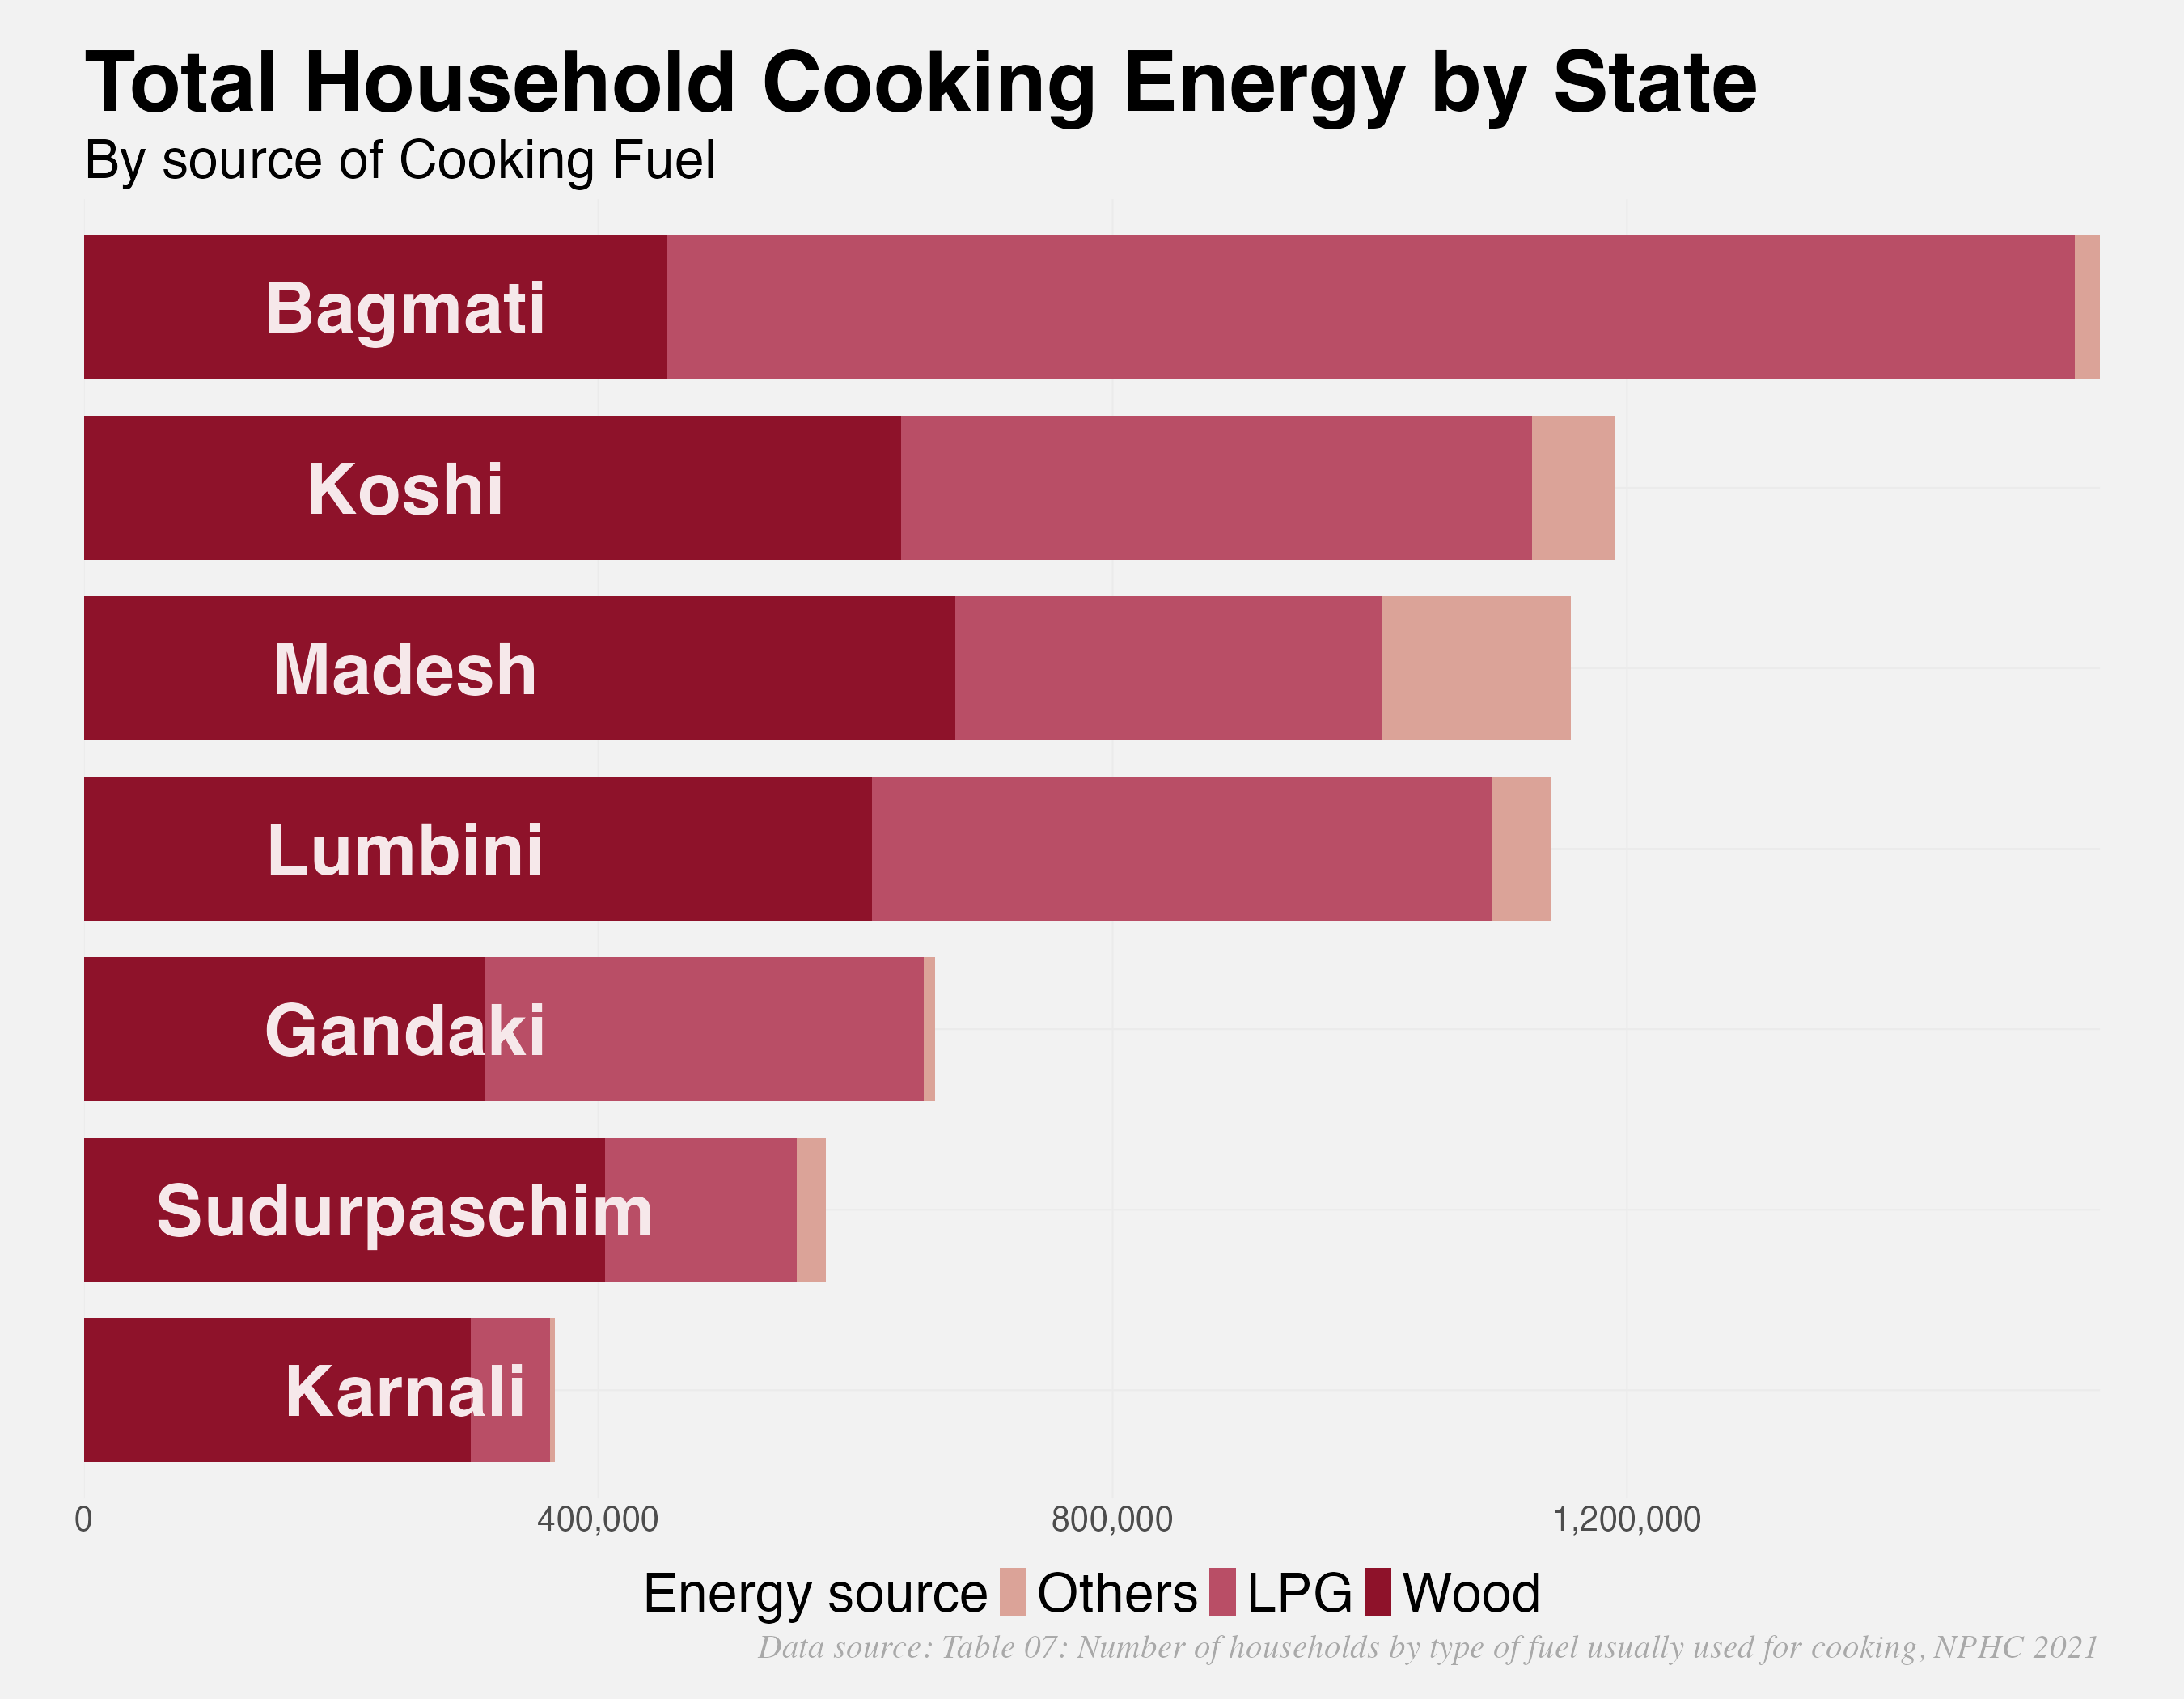
\includegraphics[width= 12 cm, height=10cm, keepaspectratio]{stacked.png}
  \caption{Cooking Energy by Province}
  \label{fig-stacked}
\end{wrapfigure}

Figure \ref{fig-stacked} shows substantial variation in cooking fuel use
across Nepal's provinces, driven largely by differences in urbanization.
Provinces with larger urban populations show higher reliance on LPG,
while more rural provinces remain dominated by wood. Bagmati Province
stands out as the most LPG-dependent region. Table~\ref{tbl-stateloc}
confirms this pattern, showing that metropolitan and sub-metropolitan
areas in Bagmati account for over 430,000 LPG-using households, compared
to fewer than 100,000 households using wood in those same urban areas.
However, this pattern reverses within rural parts of Bagmati. In
Gaunpalikas, Table~\ref{tbl-stateloc} shows that 272,337 households use
wood compared to only 72,521 using LPG, indicating that wood use remains
nearly four times higher in rural areas of the same province. In
contrast, provinces such as Karnali and Sudurpaschim are overwhelmingly
dependent on wood. We see that in Karnali's Gaunpalikas alone, 157,434
households rely on wood compared to just 8,898 households using LPG,
indicating that the vast majority of rural households still rely on
traditional fuels. These differences demonstrate that national increases
in LPG use are driven primarily by urban provinces rather than by
uniform adoption across the country.

\paragraph{Differences within
provinces}\label{differences-within-provinces}

While provincial averages reveal broad trends,
Figure~\ref{fig-stackeddist} highlights substantial variation within
provinces at the district level. Table~\ref{tbl-districtloc} indicates
that 235,688 households use LPG in Kathmandu district's metropolitan
areas compared to only 511 households using wood, meaning LPG use
exceeds wood use by more than 400 times. In contrast, nearby districts
such as Ramechhap and Sindhuli show the opposite pattern. The table
shows that wood-using households exceed LPG users by more than a tenfold
margin in these districts, reflecting much lower levels of urbanization
and infrastructure access. Similar disparities appear in other
provinces. In Jhapa District (Koshi Province), we see strong LPG use in
municipalities (123,904 households), while rural Gaunpalikas continue to
have tens of thousands of wood-using households. These patterns confirm
that vulnerability to LPG shortages is highly localized, varying
dramatically even within the same province.

\paragraph{Urban--rural divide}\label{urbanrural-divide}

\begin{wrapfigure}[25]{R}{12 cm}
  \centering
  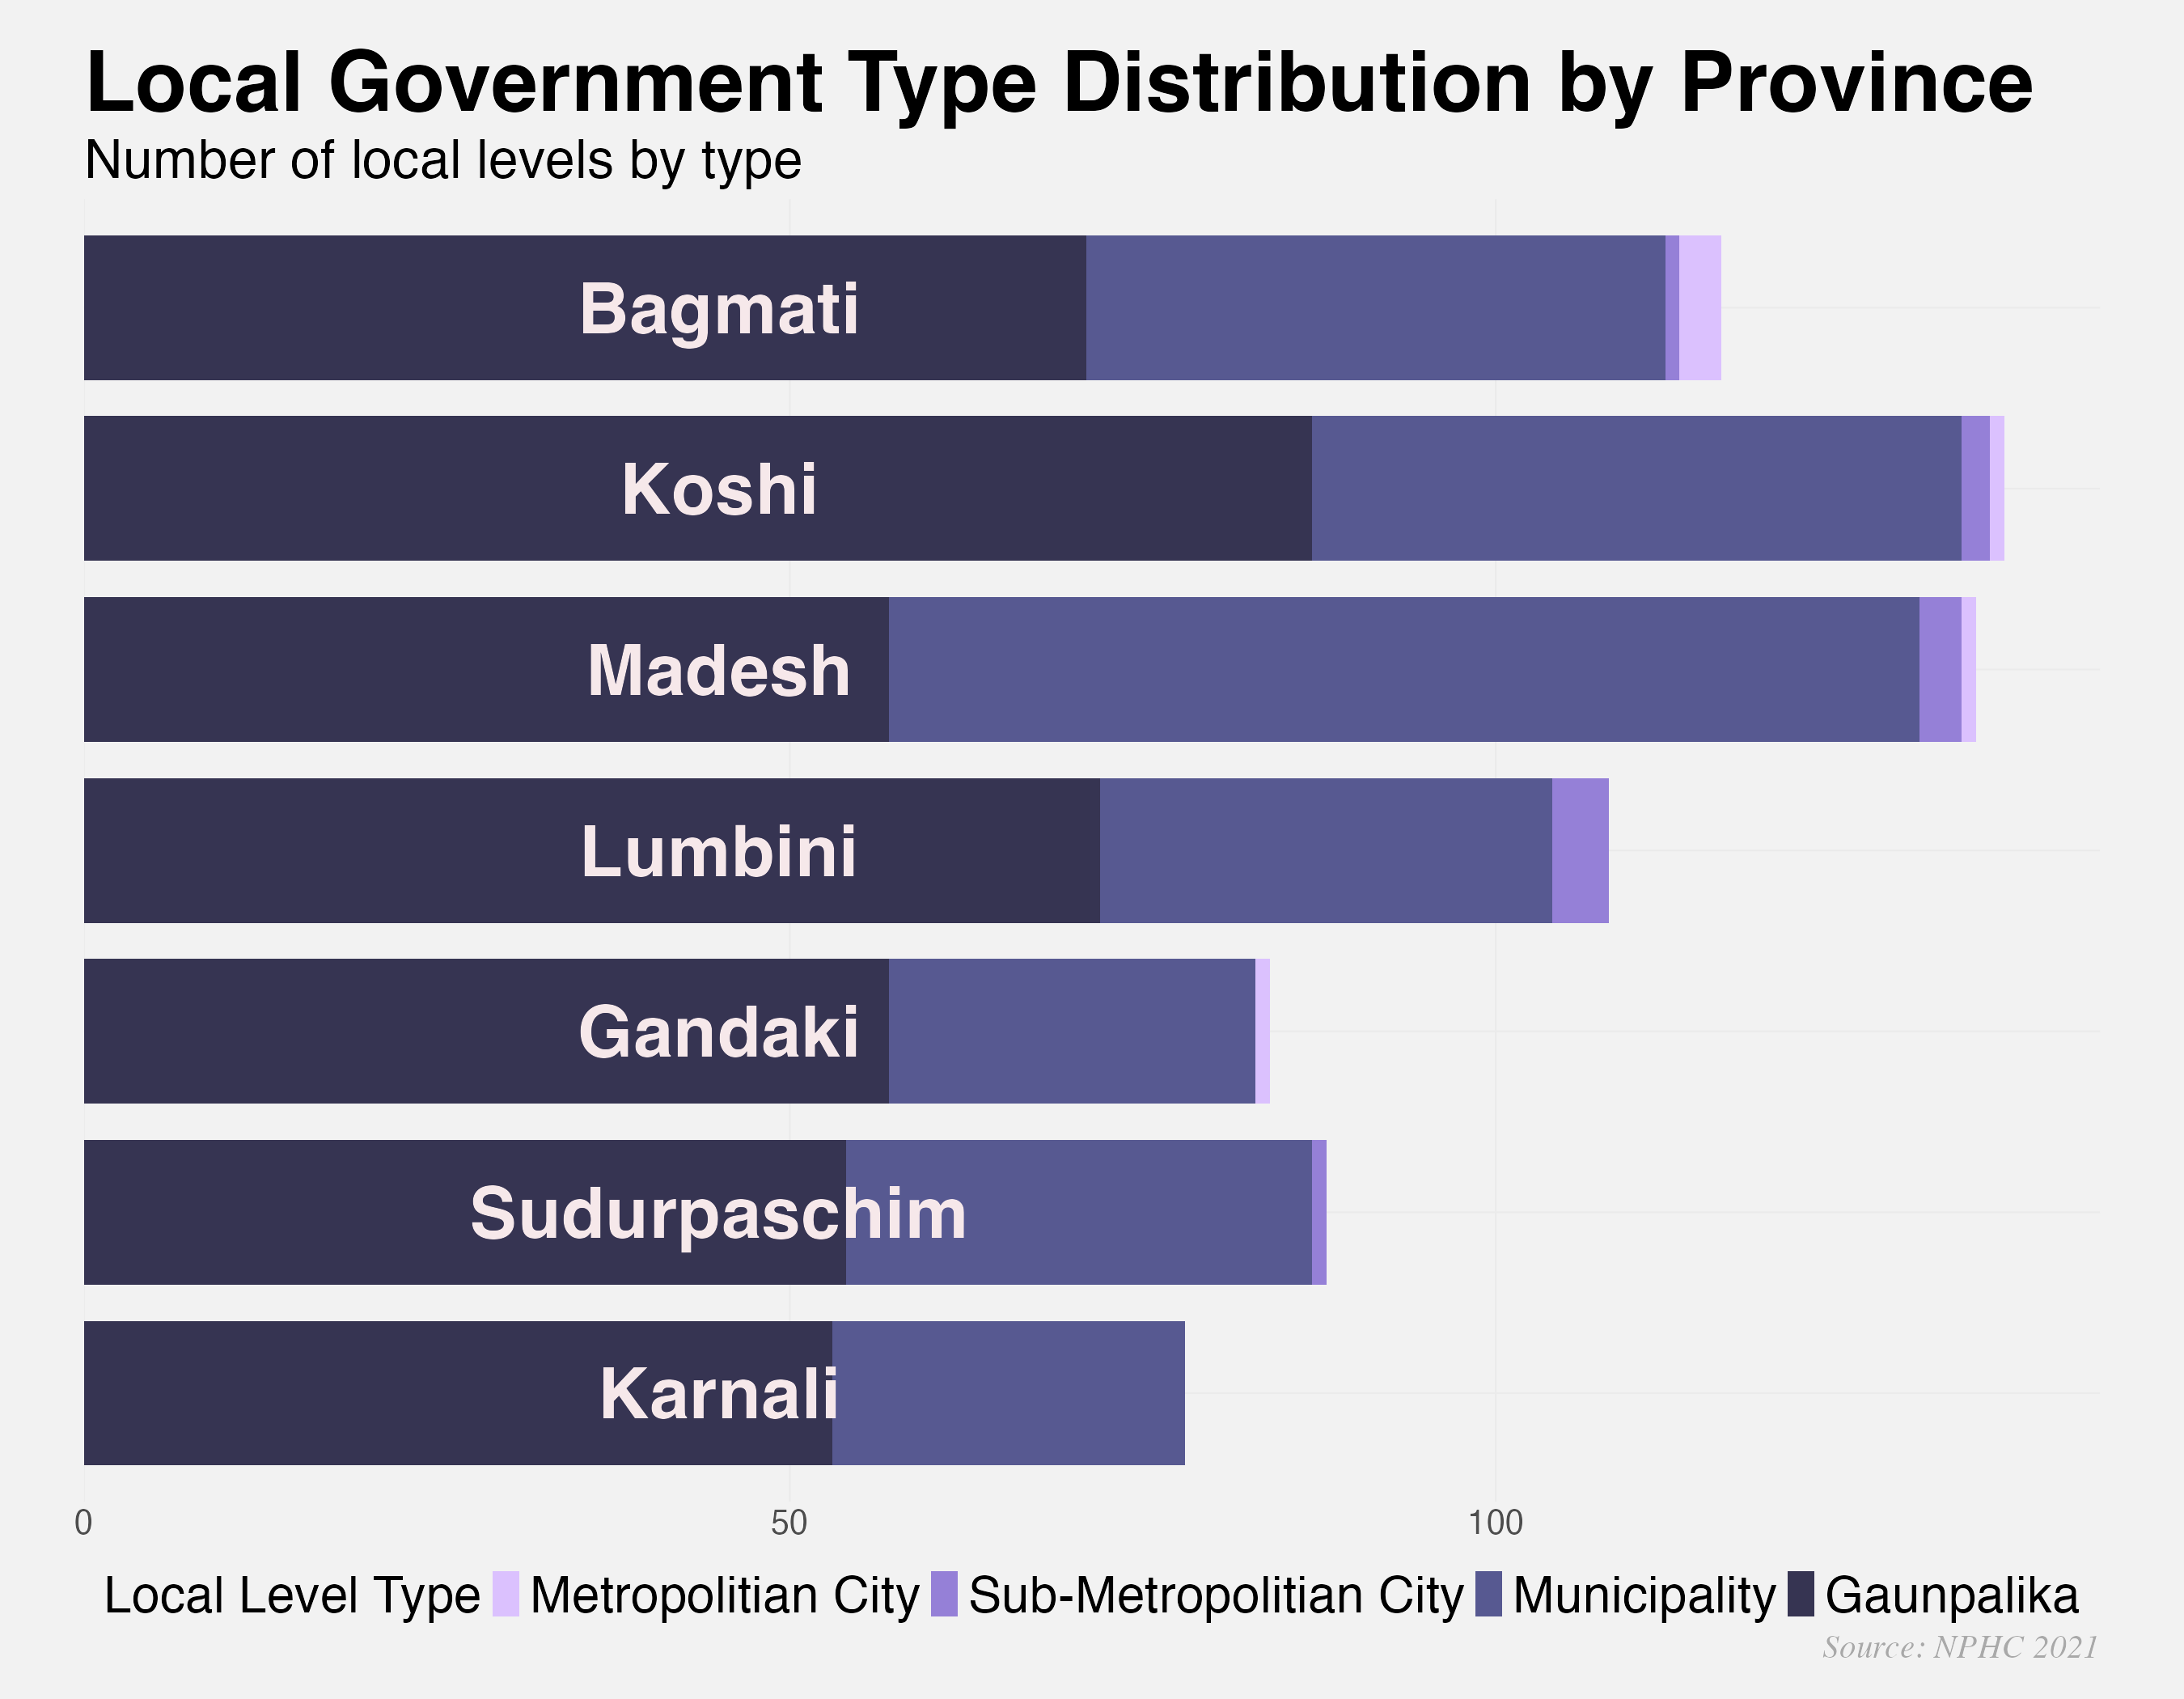
\includegraphics[width= 12 cm, height=10cm, keepaspectratio]{stacked_loctype.png}
  \caption{Local level by province}
  \label{fig-stackedmuni}
\end{wrapfigure}

Table~\ref{tbl-percentlocook} clearly demonstrates the national
urban--rural divide in cooking fuel choice, while \ref{fig-stackedmuni}
shows the share of urban and rural areas in each province based on local
government types. This helps us contextualize urban-LPG and rural-wood
pattern across provinces seen in \ref{fig-stacked}. This pattern is
consistent across provinces. For example, in Madesh Province,
Table~\ref{tbl-stateloc} shows that metropolitan areas have
significantly higher LPG use, while Gaunpalikas have 195,522 wood-using
households compared to only 51,992 LPG users, meaning wood use exceeds
LPG by nearly four times. Similarly, in Sudurpaschim, we see 183,206
households using wood compared to just 18,921 using LPG in Gaunpalikas,
indicating extremely low LPG penetration. These urban areas with LPG
dependence are also the most densely populated areas.As a result,
although rural areas rely more heavily on traditional fuels, the
majority of LPG demand, and therefore exposure to import disruptions, is
concentrated in cities and large municipalities.

\subsection{Discussion and Conclusion}\label{discussion-and-conclusion}

This analysis clarifies the core trade‑off in Nepal's cooking energy
transition. LPG adoption has delivered cleaner and faster cooking for
urban households, where over 70\% of municipal households and more than
90\% of metropolitan households rely on LPG. However, this same
concentration means that urban provinces such as Bagmati, Koshi, and
Lumbini account for the bulk of national LPG consumption, despite
representing a smaller share of total local governments. Rural areas
remain heavily dependent on wood, which reduces their exposure to global
LPG price shocks but perpetuates health and environmental risks. For
example, in Karnali and Sudurpaschim, over three‑quarters of households
still cook with wood, making LPG shortages less disruptive in the short
run but locking households into polluting fuels. Overall, the data shows
that Nepal's vulnerability to LPG supply shocks is not proportional to
population alone, but rather to urban concentration. Expanding
alternatives such as electric cooking or biogas in metropolitan and
municipal areas where LPG use exceeds wood by margins of 5:1 or more,
could substantially reduce national exposure to imported LPG while
preserving the gains from cleaner cooking.

\section{Thank you}\label{thank-you}

\section{Appendix}\label{appendix}

\begin{Shaded}
\begin{Highlighting}[]
\CommentTok{\#Setup{-}{-}{-}{-}}

\FunctionTok{library}\NormalTok{(tidyverse)}
\FunctionTok{library}\NormalTok{(knitr)}
\FunctionTok{library}\NormalTok{(kableExtra)}
\FunctionTok{library}\NormalTok{(scales)}

\CommentTok{\#Themes{-}{-}{-}{-}}
\NormalTok{mytable\_theme }\OtherTok{\textless{}{-}} \ControlFlowTok{function}\NormalTok{(table,}
                          \AttributeTok{caption =} \ConstantTok{NULL}\NormalTok{,}
                          \AttributeTok{footnote\_text =} \ConstantTok{NULL}\NormalTok{)}
\NormalTok{  table }\SpecialCharTok{|\textgreater{}}
   \FunctionTok{mutate}\NormalTok{(}
      \FunctionTok{across}\NormalTok{(}
        \FunctionTok{where}\NormalTok{(is.numeric),}
        \SpecialCharTok{\textasciitilde{}} \FunctionTok{ifelse}\NormalTok{(.x }\SpecialCharTok{==} \DecValTok{0}\NormalTok{, }\StringTok{"{-}"}\NormalTok{, .x)}
\NormalTok{      )}
\NormalTok{    ) }\SpecialCharTok{|\textgreater{}}
    \FunctionTok{kbl}\NormalTok{(}
      \AttributeTok{caption =}\NormalTok{ caption,}
      \AttributeTok{align =} \FunctionTok{c}\NormalTok{(}\StringTok{\textquotesingle{}l\textquotesingle{}}\NormalTok{, }\FunctionTok{rep}\NormalTok{(}\StringTok{\textquotesingle{}c\textquotesingle{}}\NormalTok{, }\FunctionTok{ncol}\NormalTok{(table) }\SpecialCharTok{{-}} \DecValTok{1}\NormalTok{)),}
      \AttributeTok{booktabs =} \ConstantTok{TRUE}\NormalTok{,}
      \AttributeTok{longtable =} \ConstantTok{TRUE}
\NormalTok{    ) }\SpecialCharTok{|\textgreater{}}
    \FunctionTok{kable\_styling}\NormalTok{(}
      \AttributeTok{position =} \StringTok{"center"}\NormalTok{,}
      \AttributeTok{latex\_options =} \StringTok{"hold\_position"}
\NormalTok{    ) }\SpecialCharTok{|\textgreater{}}
    \FunctionTok{row\_spec}\NormalTok{(}\DecValTok{0}\NormalTok{, }\AttributeTok{bold =} \ConstantTok{TRUE}\NormalTok{, }\AttributeTok{background =} \StringTok{"\#2E86AB"}\NormalTok{, }\AttributeTok{color =} \StringTok{"\#F2F0EF"}\NormalTok{) }\SpecialCharTok{|\textgreater{}}
    \FunctionTok{column\_spec}\NormalTok{(}\DecValTok{1}\NormalTok{, }\AttributeTok{bold =} \ConstantTok{TRUE}\NormalTok{, }\AttributeTok{background =} \StringTok{"\#F2F0EF"}\NormalTok{, }\AttributeTok{color =} \StringTok{"\#2E86AB"}\NormalTok{) }\SpecialCharTok{|\textgreater{}}
    \FunctionTok{footnote}\NormalTok{(}
      \AttributeTok{general =}\NormalTok{ footnote\_text,}
      \AttributeTok{footnote\_as\_chunk =} \ConstantTok{TRUE}\NormalTok{,}
      \AttributeTok{escape =} \ConstantTok{FALSE}\NormalTok{,}
      \AttributeTok{general\_title =} \StringTok{""}
\NormalTok{    )}

\CommentTok{\#Functions{-}{-}{-}{-}}
\NormalTok{classify\_local }\OtherTok{\textless{}{-}} \ControlFlowTok{function}\NormalTok{(data) \{}
\NormalTok{  data }\SpecialCharTok{|\textgreater{}}
    \FunctionTok{mutate}\NormalTok{(}
      \AttributeTok{Local\_type =} \FunctionTok{case\_when}\NormalTok{(}
        \FunctionTok{str\_detect}\NormalTok{(Local\_level, }\StringTok{"Gaunp"}\NormalTok{) }\SpecialCharTok{\textasciitilde{}} \StringTok{"Gaunpalika"}\NormalTok{,}
        \FunctionTok{str\_detect}\NormalTok{(Local\_level, }\StringTok{"Munici"}\NormalTok{) }\SpecialCharTok{\textasciitilde{}} \StringTok{"Municipality"}\NormalTok{,}
        \FunctionTok{str\_detect}\NormalTok{(Local\_level, }\StringTok{"Sub{-}Metro"}\NormalTok{) }\SpecialCharTok{\textasciitilde{}} \StringTok{"Sub{-}Metropolitian City"}\NormalTok{,}
        \FunctionTok{str\_detect}\NormalTok{(Local\_level, }\StringTok{"Metro"}\NormalTok{) }\SpecialCharTok{\textasciitilde{}} \StringTok{"Metropolitian City"}\NormalTok{,}
        \ConstantTok{TRUE} \SpecialCharTok{\textasciitilde{}} \StringTok{"Other"}
\NormalTok{      )}
\NormalTok{    )}
\NormalTok{\}}

\NormalTok{fuel\_summary }\OtherTok{\textless{}{-}} \ControlFlowTok{function}\NormalTok{(data, group\_var, }\AttributeTok{include\_province =} \ConstantTok{FALSE}\NormalTok{) \{}
  \ControlFlowTok{if}\NormalTok{ (include\_province) \{}
\NormalTok{    data }\SpecialCharTok{|\textgreater{}}
      \FunctionTok{classify\_local}\NormalTok{() }\SpecialCharTok{|\textgreater{}}
      \FunctionTok{group\_by}\NormalTok{(Province, \{\{ group\_var \}\}, Local\_type) }\SpecialCharTok{|\textgreater{}}
      \FunctionTok{summarise}\NormalTok{(}
        \FunctionTok{across}\NormalTok{(}\FunctionTok{c}\NormalTok{(Wood, LPG, Others), sum),}
        \AttributeTok{.groups =} \StringTok{"drop"}
\NormalTok{      ) }\SpecialCharTok{|\textgreater{}}
      \FunctionTok{arrange}\NormalTok{(}
\NormalTok{        Province, \{\{ group\_var \}\},}
        \FunctionTok{match}\NormalTok{(Local\_type, }\FunctionTok{c}\NormalTok{(}\StringTok{"Metropolitian City"}\NormalTok{, }\StringTok{"Sub{-}Metropolitian City"}\NormalTok{, }\StringTok{"Municipality"}\NormalTok{, }\StringTok{"Gaunpalika"}\NormalTok{))}
\NormalTok{      )}
\NormalTok{  \} }\ControlFlowTok{else}\NormalTok{ \{}
\NormalTok{  data }\SpecialCharTok{|\textgreater{}}
    \FunctionTok{classify\_local}\NormalTok{() }\SpecialCharTok{|\textgreater{}}
    \FunctionTok{group\_by}\NormalTok{(\{\{ group\_var \}\}, Local\_type) }\SpecialCharTok{|\textgreater{}}
    \FunctionTok{summarise}\NormalTok{(}
      \FunctionTok{across}\NormalTok{(}\FunctionTok{c}\NormalTok{(Wood, LPG, Others), sum),}
      \AttributeTok{.groups =} \StringTok{"drop"}
\NormalTok{    ) }\SpecialCharTok{|\textgreater{}}
    \FunctionTok{arrange}\NormalTok{(}
\NormalTok{      \{\{ group\_var \}\},}
      \FunctionTok{match}\NormalTok{(Local\_type, }\FunctionTok{c}\NormalTok{(}\StringTok{"Metropolitian City"}\NormalTok{, }\StringTok{"Sub{-}Metropolitian City"}\NormalTok{, }\StringTok{"Municipality"}\NormalTok{, }\StringTok{"Gaunpalika"}\NormalTok{))}
\NormalTok{    )}
\NormalTok{  \}}
\NormalTok{\}}

\NormalTok{count\_local }\OtherTok{\textless{}{-}} \ControlFlowTok{function}\NormalTok{(data, group\_var, }\AttributeTok{include\_province =} \ConstantTok{FALSE}\NormalTok{) \{}
  \ControlFlowTok{if}\NormalTok{ (include\_province) \{}
\NormalTok{    data }\SpecialCharTok{|\textgreater{}}
      \FunctionTok{classify\_local}\NormalTok{() }\SpecialCharTok{|\textgreater{}}
      \FunctionTok{distinct}\NormalTok{(Province, \{\{ group\_var \}\}, Local\_level, Local\_type) }\SpecialCharTok{|\textgreater{}}
      \FunctionTok{count}\NormalTok{(Province, \{\{ group\_var \}\}, Local\_type) }\SpecialCharTok{|\textgreater{}}
      \FunctionTok{pivot\_wider}\NormalTok{(}\AttributeTok{names\_from =}\NormalTok{ Local\_type, }\AttributeTok{values\_from =}\NormalTok{ n, }\AttributeTok{values\_fill =} \DecValTok{0}\NormalTok{) }\SpecialCharTok{|\textgreater{}}
      \FunctionTok{select}\NormalTok{(}
\NormalTok{        Province, \{\{ group\_var \}\},}
        \FunctionTok{any\_of}\NormalTok{(}\FunctionTok{c}\NormalTok{(}\StringTok{"Gaunpalika"}\NormalTok{, }\StringTok{"Municipality"}\NormalTok{, }\StringTok{"Sub{-}Metropolitian City"}\NormalTok{, }\StringTok{"Metropolitian City"}\NormalTok{))}
\NormalTok{      ) }\SpecialCharTok{|\textgreater{}}
      \FunctionTok{arrange}\NormalTok{(Province, \{\{ group\_var \}\})}
\NormalTok{  \} }\ControlFlowTok{else}\NormalTok{ \{}
\NormalTok{    data }\SpecialCharTok{|\textgreater{}}
      \FunctionTok{classify\_local}\NormalTok{() }\SpecialCharTok{|\textgreater{}}
      \FunctionTok{distinct}\NormalTok{(\{\{ group\_var \}\}, Local\_level, Local\_type) }\SpecialCharTok{|\textgreater{}}
      \FunctionTok{count}\NormalTok{(\{\{ group\_var \}\}, Local\_type) }\SpecialCharTok{|\textgreater{}}
      \FunctionTok{pivot\_wider}\NormalTok{(}\AttributeTok{names\_from =}\NormalTok{ Local\_type, }\AttributeTok{values\_from =}\NormalTok{ n, }\AttributeTok{values\_fill =} \DecValTok{0}\NormalTok{) }\SpecialCharTok{|\textgreater{}}
      \FunctionTok{select}\NormalTok{(}
\NormalTok{        \{\{ group\_var \}\},}
        \FunctionTok{any\_of}\NormalTok{(}\FunctionTok{c}\NormalTok{(}\StringTok{"Gaunpalika"}\NormalTok{, }\StringTok{"Municipality"}\NormalTok{, }\StringTok{"Sub{-}Metropolitian City"}\NormalTok{, }\StringTok{"Metropolitian City"}\NormalTok{))}
\NormalTok{      )}
\NormalTok{  \}}
\NormalTok{\}}

\NormalTok{fuel\_table }\OtherTok{\textless{}{-}} \ControlFlowTok{function}\NormalTok{(data, caption, }\AttributeTok{group\_col =} \DecValTok{1}\NormalTok{, }\AttributeTok{font =} \DecValTok{8}\NormalTok{) \{}
  \FunctionTok{mytable\_theme}\NormalTok{(}
\NormalTok{    data,}
    \AttributeTok{caption =}\NormalTok{ caption,}
    \AttributeTok{footnote\_text =} \StringTok{"Source: Census 2021."}
\NormalTok{  ) }\SpecialCharTok{|\textgreater{}}
    \FunctionTok{kable\_styling}\NormalTok{(}
      \AttributeTok{latex\_options =} \FunctionTok{c}\NormalTok{(}\StringTok{"repeat\_header"}\NormalTok{, }\StringTok{"scale\_down"}\NormalTok{),}
      \AttributeTok{font\_size =}\NormalTok{ font}
\NormalTok{    ) }\SpecialCharTok{|\textgreater{}}
    \FunctionTok{collapse\_rows}\NormalTok{(}\AttributeTok{columns =}\NormalTok{ group\_col, }\AttributeTok{valign =} \StringTok{"top"}\NormalTok{)}
\NormalTok{\}}


\CommentTok{\# Data{-}{-}{-}{-}}
\NormalTok{cooking }\OtherTok{\textless{}{-}} \FunctionTok{read.csv}\NormalTok{(}\StringTok{\textquotesingle{}Cooking\_fuel\_NP.csv\textquotesingle{}}\NormalTok{) }\SpecialCharTok{|\textgreater{}}
  \FunctionTok{mutate}\NormalTok{(}
    \AttributeTok{Others =}\NormalTok{ Electricity }\SpecialCharTok{+}\NormalTok{ Cow\_dung }\SpecialCharTok{+}\NormalTok{ Bio\_gas }\SpecialCharTok{+}\NormalTok{ Kerosene }\SpecialCharTok{+}\NormalTok{ Other}
\NormalTok{  ) }\SpecialCharTok{|\textgreater{}}
  \FunctionTok{select}\NormalTok{(Province, District, Local\_level, Total, Wood, LPG, Others )}


\NormalTok{energy\_source }\OtherTok{\textless{}{-}} \FunctionTok{c}\NormalTok{(}\StringTok{"Wood"}\NormalTok{, }\StringTok{"LPG"}\NormalTok{, }\StringTok{"Others"}\NormalTok{)}
\NormalTok{energy\_colors }\OtherTok{\textless{}{-}} \FunctionTok{c}\NormalTok{(}\AttributeTok{Wood =} \StringTok{"\#890620"}\NormalTok{, }\AttributeTok{LPG =} \StringTok{"\#b6465f"}\NormalTok{, }\AttributeTok{Others =} \StringTok{"\#da9f93"}\NormalTok{)}

\CommentTok{\#Table prep{-}{-}{-}{-}}
\NormalTok{fuel\_district }\OtherTok{\textless{}{-}} \FunctionTok{fuel\_summary}\NormalTok{(cooking, District, }\AttributeTok{include\_province =} \ConstantTok{TRUE}\NormalTok{)}
\NormalTok{fuel\_state }\OtherTok{\textless{}{-}} \FunctionTok{fuel\_summary}\NormalTok{(cooking, Province)}
\NormalTok{count\_dist }\OtherTok{\textless{}{-}} \FunctionTok{count\_local}\NormalTok{(cooking, District, }\AttributeTok{include\_province =} \ConstantTok{TRUE}\NormalTok{)}
\NormalTok{count\_prov }\OtherTok{\textless{}{-}} \FunctionTok{count\_local}\NormalTok{(cooking, Province)}

\NormalTok{province\_order }\OtherTok{\textless{}{-}}\NormalTok{ cooking }\SpecialCharTok{|\textgreater{}}
  \FunctionTok{group\_by}\NormalTok{(Province) }\SpecialCharTok{|\textgreater{}}
  \FunctionTok{summarise}\NormalTok{(}\AttributeTok{total =} \FunctionTok{sum}\NormalTok{(Total)) }\SpecialCharTok{|\textgreater{}}
  \FunctionTok{arrange}\NormalTok{(total) }\SpecialCharTok{|\textgreater{}}
  \FunctionTok{pull}\NormalTok{(Province)}
\end{Highlighting}
\end{Shaded}

\begin{Shaded}
\begin{Highlighting}[]
\NormalTok{energy\_df\_prov }\OtherTok{\textless{}{-}}\NormalTok{ cooking }\SpecialCharTok{|\textgreater{}}
  \FunctionTok{select}\NormalTok{(Province, }\FunctionTok{all\_of}\NormalTok{(energy\_source))}

\NormalTok{barplot\_province }\OtherTok{\textless{}{-}} \FunctionTok{aggregate}\NormalTok{(}
\NormalTok{  energy\_df\_prov[, energy\_source],}
  \AttributeTok{by =} \FunctionTok{list}\NormalTok{(}\AttributeTok{Province =}\NormalTok{ energy\_df\_prov}\SpecialCharTok{$}\NormalTok{Province),}
\NormalTok{  sum}
\NormalTok{) }\SpecialCharTok{|\textgreater{}}
  \FunctionTok{pivot\_longer}\NormalTok{(}
    \AttributeTok{cols =} \FunctionTok{all\_of}\NormalTok{(energy\_source),}
    \AttributeTok{names\_to =} \StringTok{"Source"}\NormalTok{,}
    \AttributeTok{values\_to =} \StringTok{"NumHouse"}
\NormalTok{  ) }\SpecialCharTok{|\textgreater{}}
  \FunctionTok{group\_by}\NormalTok{(Province) }\SpecialCharTok{|\textgreater{}}
  \FunctionTok{mutate}\NormalTok{(}\AttributeTok{total =} \FunctionTok{sum}\NormalTok{(NumHouse)) }\SpecialCharTok{|\textgreater{}}
  \FunctionTok{ungroup}\NormalTok{() }\SpecialCharTok{|\textgreater{}}
  \FunctionTok{mutate}\NormalTok{(}
    \AttributeTok{Province =} \FunctionTok{factor}\NormalTok{(Province, }\AttributeTok{levels =}\NormalTok{ province\_order),}
    \AttributeTok{Source =} \FunctionTok{fct\_reorder}\NormalTok{(Source, NumHouse, sum)}
\NormalTok{  )}

\NormalTok{stacked }\OtherTok{\textless{}{-}}\NormalTok{ barplot\_province }\SpecialCharTok{|\textgreater{}}
  \FunctionTok{ggplot}\NormalTok{(}\FunctionTok{aes}\NormalTok{(}
    \AttributeTok{x =}\NormalTok{ NumHouse,}
    \AttributeTok{y =}\NormalTok{ Province,}
    \AttributeTok{fill =}\NormalTok{ Source}
\NormalTok{  )) }\SpecialCharTok{+}
  \FunctionTok{geom\_bar}\NormalTok{(}
    \AttributeTok{width =} \FloatTok{0.8}\NormalTok{,}
    \AttributeTok{stat =} \StringTok{"identity"}\NormalTok{,}
    \AttributeTok{position =} \StringTok{"stack"}\NormalTok{,}
    \AttributeTok{alpha =} \FloatTok{0.95}
\NormalTok{  ) }\SpecialCharTok{+}
  \FunctionTok{geom\_text}\NormalTok{(}
    \AttributeTok{data =} \FunctionTok{distinct}\NormalTok{(barplot\_province, Province, total),}
    \FunctionTok{aes}\NormalTok{(}
      \AttributeTok{x =} \DecValTok{250000}\NormalTok{,}
      \AttributeTok{y =}\NormalTok{ Province,}
      \AttributeTok{label =}\NormalTok{ Province}
\NormalTok{    ),}
    \AttributeTok{inherit.aes =} \ConstantTok{FALSE}\NormalTok{,}
    \AttributeTok{color =} \StringTok{"\#f6e8ea"}\NormalTok{,}
   \AttributeTok{size =} \DecValTok{15}\NormalTok{,}
    \AttributeTok{fontface =} \StringTok{"bold"}
\NormalTok{  ) }\SpecialCharTok{+}
  \FunctionTok{scale\_fill\_manual}\NormalTok{(}\AttributeTok{values =}\NormalTok{ energy\_colors) }\SpecialCharTok{+}
  \FunctionTok{scale\_x\_continuous}\NormalTok{(}
    \AttributeTok{labels =}\NormalTok{ scales}\SpecialCharTok{::}\NormalTok{comma,}
    \AttributeTok{expand =} \FunctionTok{expansion}\NormalTok{(}\AttributeTok{mult =} \FunctionTok{c}\NormalTok{(}\DecValTok{0}\NormalTok{, }\DecValTok{0}\NormalTok{))}
\NormalTok{  ) }\SpecialCharTok{+}
  \FunctionTok{labs}\NormalTok{(}
    \AttributeTok{title =} \StringTok{"Total Household Cooking Energy by State"}\NormalTok{,}
    \AttributeTok{subtitle =} \StringTok{"By source of Cooking Fuel"}\NormalTok{,}
    \AttributeTok{fill =} \StringTok{"Energy source"}\NormalTok{,}
    \AttributeTok{caption =} \StringTok{"Data source: Table 07: Number of households by type of fuel usually used for cooking, NPHC 2021"}
\NormalTok{  ) }\SpecialCharTok{+}
  \FunctionTok{theme\_minimal}\NormalTok{() }\SpecialCharTok{+}
  \FunctionTok{theme}\NormalTok{(}
    \AttributeTok{plot.title =} \FunctionTok{element\_text}\NormalTok{(}\AttributeTok{size =} \DecValTok{50}\NormalTok{, }\AttributeTok{hjust =} \DecValTok{0}\NormalTok{, }\AttributeTok{face =} \StringTok{"bold"}\NormalTok{, }\AttributeTok{family =} \StringTok{"sans"}\NormalTok{),}
    \AttributeTok{plot.title.position =} \StringTok{"plot"}\NormalTok{,}
    \AttributeTok{plot.subtitle =} \FunctionTok{element\_text}\NormalTok{(}\AttributeTok{hjust =} \DecValTok{0}\NormalTok{, }\AttributeTok{size =} \DecValTok{32}\NormalTok{, }\AttributeTok{family =} \StringTok{"sans"}\NormalTok{),}
    \AttributeTok{plot.background =} \FunctionTok{element\_rect}\NormalTok{(}\AttributeTok{fill =} \StringTok{"\#f2f2f2"}\NormalTok{, }\AttributeTok{color =} \ConstantTok{NA}\NormalTok{),}
    \AttributeTok{panel.grid.minor =} \FunctionTok{element\_blank}\NormalTok{(),}
    \AttributeTok{axis.title =} \FunctionTok{element\_blank}\NormalTok{(),}
    \AttributeTok{axis.text.y =} \FunctionTok{element\_blank}\NormalTok{(),}
    \AttributeTok{axis.text.x =} \FunctionTok{element\_text}\NormalTok{(}\AttributeTok{size =} \DecValTok{20}\NormalTok{),}
    \AttributeTok{axis.ticks.y =} \FunctionTok{element\_blank}\NormalTok{(),}
    \AttributeTok{plot.caption.position =} \StringTok{"plot"}\NormalTok{,}
    \AttributeTok{plot.caption =} \FunctionTok{element\_text}\NormalTok{(}\AttributeTok{hjust =} \DecValTok{1}\NormalTok{, }\AttributeTok{size =} \DecValTok{20}\NormalTok{, }\AttributeTok{face =} \StringTok{"italic"}\NormalTok{, }\AttributeTok{family =} \StringTok{"times"}\NormalTok{, }\AttributeTok{color =} \StringTok{\textquotesingle{}darkgray\textquotesingle{}}\NormalTok{),}
    \AttributeTok{legend.position =} \StringTok{"bottom"}\NormalTok{,}
    \AttributeTok{legend.text =} \FunctionTok{element\_text}\NormalTok{(}\AttributeTok{size =} \DecValTok{32}\NormalTok{),}
    \AttributeTok{legend.title =} \FunctionTok{element\_text}\NormalTok{(}\AttributeTok{size =} \DecValTok{32}\NormalTok{),}
    \AttributeTok{plot.margin =} \FunctionTok{margin}\NormalTok{(}\AttributeTok{t =} \DecValTok{30}\NormalTok{, }\AttributeTok{r =} \DecValTok{50}\NormalTok{, }\AttributeTok{b =} \DecValTok{20}\NormalTok{, }\AttributeTok{l =} \DecValTok{50}\NormalTok{, }\AttributeTok{unit =} \StringTok{"pt"}\NormalTok{)}
\NormalTok{  )}

\FunctionTok{ggsave}\NormalTok{(}\StringTok{"stacked.png"}\NormalTok{, }\AttributeTok{plot =}\NormalTok{ stacked, }\AttributeTok{width =} \DecValTok{18}\NormalTok{, }\AttributeTok{height =} \DecValTok{14}\NormalTok{, }\AttributeTok{dpi =} \DecValTok{150}\NormalTok{)}
\end{Highlighting}
\end{Shaded}

\begin{Shaded}
\begin{Highlighting}[]
\NormalTok{energy\_df\_dist }\OtherTok{\textless{}{-}}\NormalTok{ cooking }\SpecialCharTok{|\textgreater{}}
  \FunctionTok{select}\NormalTok{(Province, District, }\FunctionTok{all\_of}\NormalTok{(energy\_source))}

\NormalTok{barplot\_district }\OtherTok{\textless{}{-}} \FunctionTok{aggregate}\NormalTok{(}
\NormalTok{    energy\_df\_dist[, energy\_source],}
    \AttributeTok{by =} \FunctionTok{list}\NormalTok{(}\AttributeTok{Province =}\NormalTok{ energy\_df\_dist}\SpecialCharTok{$}\NormalTok{Province, }\AttributeTok{District =}\NormalTok{ energy\_df\_dist}\SpecialCharTok{$}\NormalTok{District),}
\NormalTok{    sum}
\NormalTok{  ) }\SpecialCharTok{|\textgreater{}}
  \FunctionTok{pivot\_longer}\NormalTok{(}
    \AttributeTok{cols =} \FunctionTok{all\_of}\NormalTok{(energy\_source),}
    \AttributeTok{names\_to =} \StringTok{"Source"}\NormalTok{,}
    \AttributeTok{values\_to =} \StringTok{"NumHouse"}
\NormalTok{  ) }\SpecialCharTok{|\textgreater{}}
  \FunctionTok{group\_by}\NormalTok{(District) }\SpecialCharTok{|\textgreater{}}
  \FunctionTok{mutate}\NormalTok{(}\AttributeTok{total =} \FunctionTok{sum}\NormalTok{(NumHouse)) }\SpecialCharTok{|\textgreater{}}
  \FunctionTok{ungroup}\NormalTok{() }\SpecialCharTok{|\textgreater{}}
  \FunctionTok{mutate}\NormalTok{(}
    \AttributeTok{Province =} \FunctionTok{factor}\NormalTok{(Province, }\AttributeTok{levels =}\NormalTok{ province\_order),}
    \AttributeTok{District =} \FunctionTok{fct\_reorder}\NormalTok{(District, total),}
    \AttributeTok{Source =} \FunctionTok{fct\_reorder}\NormalTok{(Source, NumHouse, sum),}
    \AttributeTok{label\_hjust =} \FloatTok{1.20}\NormalTok{,}
    \AttributeTok{label\_color =} \StringTok{"\#f6e8ea"}
\NormalTok{  )}

\NormalTok{stacked\_districts }\OtherTok{\textless{}{-}}\NormalTok{ barplot\_district }\SpecialCharTok{|\textgreater{}}
  \FunctionTok{ggplot}\NormalTok{(}\FunctionTok{aes}\NormalTok{(}\AttributeTok{x =}\NormalTok{ NumHouse, }\AttributeTok{y =}\NormalTok{ District, }\AttributeTok{fill =}\NormalTok{ Source)) }\SpecialCharTok{+}
  \FunctionTok{geom\_bar}\NormalTok{(}\AttributeTok{stat =} \StringTok{"identity"}\NormalTok{, }\AttributeTok{position =} \StringTok{"stack"}\NormalTok{, }\AttributeTok{alpha =} \FloatTok{0.95}\NormalTok{) }\SpecialCharTok{+}
  \FunctionTok{geom\_label}\NormalTok{(}
    \AttributeTok{data =} \FunctionTok{distinct}\NormalTok{(barplot\_district, District, Province, total,  }
\NormalTok{                    label\_hjust, label\_color),}
\FunctionTok{aes}\NormalTok{(}
  \AttributeTok{x =} \DecValTok{350000}\NormalTok{,}
  \AttributeTok{y =}\NormalTok{ District,}
  \AttributeTok{label =}\NormalTok{ District),}
\AttributeTok{size =} \DecValTok{6}\NormalTok{,}
\AttributeTok{fill =} \StringTok{\textquotesingle{}\#FAECEC\textquotesingle{}}\NormalTok{,}
\AttributeTok{color =} \StringTok{\textquotesingle{}black\textquotesingle{}}\NormalTok{,}
\AttributeTok{style =} \StringTok{\textquotesingle{}bold\textquotesingle{}}\NormalTok{,}
\AttributeTok{inherit.aes =} \ConstantTok{FALSE}
\NormalTok{  ) }\SpecialCharTok{+}
  \FunctionTok{scale\_color\_identity}\NormalTok{() }\SpecialCharTok{+}
  \FunctionTok{scale\_fill\_manual}\NormalTok{(}\AttributeTok{values =}\NormalTok{ energy\_colors) }\SpecialCharTok{+}
  \FunctionTok{scale\_x\_continuous}\NormalTok{(}
    \AttributeTok{labels =}\NormalTok{ scales}\SpecialCharTok{::}\NormalTok{comma,}
    \AttributeTok{expand =} \FunctionTok{expansion}\NormalTok{(}\AttributeTok{mult =} \FunctionTok{c}\NormalTok{(}\DecValTok{0}\NormalTok{, }\FloatTok{0.35}\NormalTok{))}
\NormalTok{  ) }\SpecialCharTok{+}
  \FunctionTok{facet\_wrap}\NormalTok{(}\SpecialCharTok{\textasciitilde{}}\NormalTok{ Province, }\AttributeTok{scales =} \StringTok{"free\_y"}\NormalTok{, }\AttributeTok{ncol =} \DecValTok{2}\NormalTok{) }\SpecialCharTok{+}
  \FunctionTok{labs}\NormalTok{(}
    \AttributeTok{title  =} \StringTok{"Total Household Cooking Energy by District"}\NormalTok{,}
    \AttributeTok{subtitle =} \StringTok{"By source of Cooking Fuel"}\NormalTok{,}
    \AttributeTok{fill  =} \StringTok{"Energy Source"}\NormalTok{,}
    \AttributeTok{caption =} \StringTok{"Data source: Table 07: Number of households by type of fuel usually used for cooking, NPHC 2021"}
\NormalTok{  ) }\SpecialCharTok{+}
  \FunctionTok{theme\_minimal}\NormalTok{() }\SpecialCharTok{+}
  \FunctionTok{theme}\NormalTok{(}
    \AttributeTok{plot.title =} \FunctionTok{element\_text}\NormalTok{(}\AttributeTok{size =} \DecValTok{42}\NormalTok{, }\AttributeTok{hjust =} \DecValTok{0}\NormalTok{, }\AttributeTok{face =} \StringTok{"bold"}\NormalTok{, }\AttributeTok{family =} \StringTok{"sans"}\NormalTok{),}
    \AttributeTok{plot.title.position =} \StringTok{"plot"}\NormalTok{,}
    \AttributeTok{plot.subtitle  =} \FunctionTok{element\_text}\NormalTok{(}\AttributeTok{hjust =} \DecValTok{0}\NormalTok{, }\AttributeTok{size =} \DecValTok{30}\NormalTok{, }\AttributeTok{family =} \StringTok{"sans"}\NormalTok{),}
    \AttributeTok{plot.background =} \FunctionTok{element\_rect}\NormalTok{(}\AttributeTok{fill =} \StringTok{"\#F2F0EF"}\NormalTok{, }\AttributeTok{color =} \ConstantTok{NA}\NormalTok{),}
    \AttributeTok{panel.grid.minor =} \FunctionTok{element\_blank}\NormalTok{(),}
    \AttributeTok{axis.title  =} \FunctionTok{element\_blank}\NormalTok{(),}
    \AttributeTok{axis.text.y =} \FunctionTok{element\_blank}\NormalTok{(),}
    \AttributeTok{axis.text.x =} \FunctionTok{element\_text}\NormalTok{(}\AttributeTok{size =} \DecValTok{18}\NormalTok{),}
    \AttributeTok{axis.ticks.y=} \FunctionTok{element\_blank}\NormalTok{(),}
 \AttributeTok{plot.caption.position =} \StringTok{"plot"}\NormalTok{,}
    \AttributeTok{plot.caption  =} \FunctionTok{element\_text}\NormalTok{(}\AttributeTok{hjust =} \DecValTok{1}\NormalTok{, }\AttributeTok{face =} \StringTok{"italic"}\NormalTok{, }\AttributeTok{family =} \StringTok{"sans"}\NormalTok{, }\AttributeTok{size =} \DecValTok{18}\NormalTok{, }\AttributeTok{color=} \StringTok{\textquotesingle{}darkgray\textquotesingle{}}\NormalTok{),}
    \AttributeTok{strip.text =} \FunctionTok{element\_text}\NormalTok{(}\AttributeTok{hjust =} \FloatTok{0.47}\NormalTok{, }\AttributeTok{size =} \DecValTok{22}\NormalTok{, }\AttributeTok{face =} \StringTok{"bold"}\NormalTok{),}
\AttributeTok{legend.position =} \StringTok{"top"}\NormalTok{,}
     \AttributeTok{legend.text =} \FunctionTok{element\_text}\NormalTok{(}\AttributeTok{size =} \DecValTok{20}\NormalTok{),}
    \AttributeTok{legend.title =} \FunctionTok{element\_text}\NormalTok{(}\AttributeTok{size =} \DecValTok{19}\NormalTok{),}
 \AttributeTok{plot.margin =} \FunctionTok{margin}\NormalTok{(}\AttributeTok{t =} \DecValTok{30}\NormalTok{, }\AttributeTok{r =} \DecValTok{20}\NormalTok{, }\AttributeTok{b =} \DecValTok{20}\NormalTok{, }\AttributeTok{l =} \DecValTok{20}\NormalTok{, }\AttributeTok{unit =} \StringTok{"pt"}\NormalTok{)}
\NormalTok{  )}

\FunctionTok{ggsave}\NormalTok{(}\StringTok{"stacked\_districts.png"}\NormalTok{, }\AttributeTok{plot =}\NormalTok{ stacked\_districts, }\AttributeTok{width =} \DecValTok{20}\NormalTok{, }\AttributeTok{height =} \DecValTok{26}\NormalTok{, }\AttributeTok{dpi =} \DecValTok{150}\NormalTok{)}
\end{Highlighting}
\end{Shaded}

\begin{Shaded}
\begin{Highlighting}[]
\FunctionTok{fuel\_table}\NormalTok{(fuel\_state, }\StringTok{"Cooking Fuel by Local Level Type per State"}\NormalTok{, }\AttributeTok{font =} \DecValTok{7}\NormalTok{)}
\end{Highlighting}
\end{Shaded}

\begingroup\fontsize{7}{9}\selectfont

\begin{longtable}[t]{>{}lcccc}

\caption{\label{tbl-stateloc}Cooking Fuel by Local Level Type per State}

\tabularnewline

\\
\toprule
\cellcolor[HTML]{2E86AB}{\textcolor[HTML]{F2F0EF}{\textbf{Province}}} & \cellcolor[HTML]{2E86AB}{\textcolor[HTML]{F2F0EF}{\textbf{Local\_type}}} & \cellcolor[HTML]{2E86AB}{\textcolor[HTML]{F2F0EF}{\textbf{Wood}}} & \cellcolor[HTML]{2E86AB}{\textcolor[HTML]{F2F0EF}{\textbf{LPG}}} & \cellcolor[HTML]{2E86AB}{\textcolor[HTML]{F2F0EF}{\textbf{Others}}}\\
\midrule
\endfirsthead
\caption[]{Cooking Fuel by Local Level Type per State \textit{(continued)}}\\
\toprule
\cellcolor[HTML]{2E86AB}{\textcolor[HTML]{F2F0EF}{\textbf{Province}}} & \cellcolor[HTML]{2E86AB}{\textcolor[HTML]{F2F0EF}{\textbf{Local\_type}}} & \cellcolor[HTML]{2E86AB}{\textcolor[HTML]{F2F0EF}{\textbf{Wood}}} & \cellcolor[HTML]{2E86AB}{\textcolor[HTML]{F2F0EF}{\textbf{LPG}}} & \cellcolor[HTML]{2E86AB}{\textcolor[HTML]{F2F0EF}{\textbf{Others}}}\\
\midrule
\endhead

\endfoot
\bottomrule
\endlastfoot
 & Metropolitian City & 13705 & 392880 & 6131\\
\cmidrule{2-5}\nopagebreak
 & Sub-Metropolitian City & 8122 & 37806 & 638\\
\cmidrule{2-5}\nopagebreak
 & Municipality & 159823 & 590988 & 9880\\
\cmidrule{2-5}\nopagebreak
\multirow[t]{-4}{*}{\raggedright\arraybackslash \cellcolor[HTML]{F2F0EF}{\textcolor[HTML]{2E86AB}{\textbf{Bagmati}}}} & Gaunpalika & 272337 & 72521 & 3086\\
\cmidrule{1-5}\pagebreak[0]
 & Metropolitian City & 11893 & 127571 & 995\\
\cmidrule{2-5}\nopagebreak
 & Municipality & 133272 & 158515 & 4986\\
\cmidrule{2-5}\nopagebreak
\multirow[t]{-3}{*}{\raggedright\arraybackslash \cellcolor[HTML]{F2F0EF}{\textcolor[HTML]{2E86AB}{\textbf{Gandaki}}}} & Gaunpalika & 166760 & 54931 & 2709\\
\cmidrule{1-5}\pagebreak[0]
 & Municipality & 143528 & 52829 & 2092\\
\cmidrule{2-5}\nopagebreak
\multirow[t]{-2}{*}{\raggedright\arraybackslash \cellcolor[HTML]{F2F0EF}{\textcolor[HTML]{2E86AB}{\textbf{Karnali}}}} & Gaunpalika & 157434 & 8898 & 1256\\
\cmidrule{1-5}\pagebreak[0]
 & Metropolitian City & 9270 & 45657 & 1992\\
\cmidrule{2-5}\nopagebreak
 & Sub-Metropolitian City & 12827 & 78541 & 1378\\
\cmidrule{2-5}\nopagebreak
 & Municipality & 294795 & 287077 & 23957\\
\cmidrule{2-5}\nopagebreak
\multirow[t]{-4}{*}{\raggedright\arraybackslash \cellcolor[HTML]{F2F0EF}{\textcolor[HTML]{2E86AB}{\textbf{Koshi}}}} & Gaunpalika & 318780 & 79022 & 37459\\
\cmidrule{1-5}\pagebreak[0]
 & Sub-Metropolitian City & 52433 & 124493 & 3983\\
\cmidrule{2-5}\nopagebreak
 & Municipality & 215319 & 230168 & 19554\\
\cmidrule{2-5}\nopagebreak
\multirow[t]{-3}{*}{\raggedright\arraybackslash \cellcolor[HTML]{F2F0EF}{\textcolor[HTML]{2E86AB}{\textbf{Lumbini}}}} & Gaunpalika & 344946 & 127087 & 23362\\
\cmidrule{1-5}\pagebreak[0]
 & Metropolitian City & 11020 & 35580 & 514\\
\cmidrule{2-5}\nopagebreak
 & Sub-Metropolitian City & 32358 & 52266 & 3560\\
\cmidrule{2-5}\nopagebreak
 & Municipality & 438832 & 192154 & 84055\\
\cmidrule{2-5}\nopagebreak
\multirow[t]{-4}{*}{\raggedright\arraybackslash \cellcolor[HTML]{F2F0EF}{\textcolor[HTML]{2E86AB}{\textbf{Madesh}}}} & Gaunpalika & 195522 & 51992 & 58530\\
\cmidrule{1-5}\pagebreak[0]
 & Sub-Metropolitian City & 13952 & 29261 & 1566\\
\cmidrule{2-5}\nopagebreak
 & Municipality & 208182 & 100837 & 13464\\
\cmidrule{2-5}\nopagebreak
\multirow[t]{-3}{*}{\raggedright\arraybackslash \cellcolor[HTML]{F2F0EF}{\textcolor[HTML]{2E86AB}{\textbf{Sudurpaschim}}}} & Gaunpalika & 183206 & 18921 & 7383\\*
\multicolumn{5}{l}{\rule{0pt}{1em}Source: Census 2021.}\\

\end{longtable}

\endgroup{}

\begin{Shaded}
\begin{Highlighting}[]
\NormalTok{fuel\_percent }\OtherTok{\textless{}{-}} \FunctionTok{fuel\_summary}\NormalTok{(cooking, Province) }\SpecialCharTok{|\textgreater{}}
  \FunctionTok{group\_by}\NormalTok{(Local\_type) }\SpecialCharTok{|\textgreater{}}
  \FunctionTok{summarise}\NormalTok{(}
    \FunctionTok{across}\NormalTok{(}\FunctionTok{c}\NormalTok{(Wood, LPG, Others), sum),}
    \AttributeTok{Total =} \FunctionTok{sum}\NormalTok{(Wood, LPG, Others),}
    \AttributeTok{.groups =} \StringTok{"drop"}
\NormalTok{  ) }\SpecialCharTok{|\textgreater{}}
  \FunctionTok{mutate}\NormalTok{(}
    \AttributeTok{National\_total =} \FunctionTok{sum}\NormalTok{(Total),}
    \AttributeTok{National\_Share =} \FunctionTok{round}\NormalTok{((Total }\SpecialCharTok{/}\NormalTok{ National\_total) }\SpecialCharTok{*} \DecValTok{100}\NormalTok{, }\DecValTok{1}\NormalTok{),}
    \FunctionTok{across}\NormalTok{(}\FunctionTok{c}\NormalTok{(Wood, LPG, Others),}
           \SpecialCharTok{\textasciitilde{}} \FunctionTok{round}\NormalTok{(.x }\SpecialCharTok{/}\NormalTok{ Total }\SpecialCharTok{*} \DecValTok{100}\NormalTok{, }\DecValTok{1}\NormalTok{)),}
    \FunctionTok{across}\NormalTok{(}
      \SpecialCharTok{{-}}\NormalTok{Local\_type,}
      \SpecialCharTok{\textasciitilde{}} \FunctionTok{paste0}\NormalTok{(.x, }\StringTok{"\%"}\NormalTok{)}
\NormalTok{    )}
\NormalTok{  ) }\SpecialCharTok{|\textgreater{}}
  \FunctionTok{select}\NormalTok{(}
\NormalTok{    Local\_type, National\_Share,}
\NormalTok{    Wood, LPG, Others}
\NormalTok{  ) }\SpecialCharTok{|\textgreater{}}
  \FunctionTok{arrange}\NormalTok{(}\FunctionTok{match}\NormalTok{(Local\_type,}
                \FunctionTok{c}\NormalTok{(}\StringTok{"Metropolitian City"}\NormalTok{,}
                  \StringTok{"Sub{-}Metropolitian City"}\NormalTok{,}
                  \StringTok{"Municipality"}\NormalTok{,}
                  \StringTok{"Gaunpalika"}\NormalTok{)))}
\end{Highlighting}
\end{Shaded}

\begin{Shaded}
\begin{Highlighting}[]
\FunctionTok{fuel\_table}\NormalTok{(fuel\_percent, }\StringTok{"Percentage Distribution of Cooking Fuel by Local Level Type"}\NormalTok{)}
\end{Highlighting}
\end{Shaded}

\begin{Shaded}
\begin{Highlighting}[]
\FunctionTok{fuel\_table}\NormalTok{(fuel\_district, }\StringTok{"Cooking Fuel by Local Level Type per District"}\NormalTok{,}
           \AttributeTok{group\_col =} \FunctionTok{c}\NormalTok{(}\DecValTok{1}\NormalTok{,}\DecValTok{2}\NormalTok{),}
           \AttributeTok{font =} \DecValTok{7}\NormalTok{)}
\end{Highlighting}
\end{Shaded}

\begingroup\fontsize{7}{9}\selectfont

\begin{longtable}[t]{>{}lccccc}

\caption{\label{tbl-districtloc}Cooking Fuel by Local Level Type per
District}

\tabularnewline

\\
\toprule
\cellcolor[HTML]{2E86AB}{\textcolor[HTML]{F2F0EF}{\textbf{Province}}} & \cellcolor[HTML]{2E86AB}{\textcolor[HTML]{F2F0EF}{\textbf{District}}} & \cellcolor[HTML]{2E86AB}{\textcolor[HTML]{F2F0EF}{\textbf{Local\_type}}} & \cellcolor[HTML]{2E86AB}{\textcolor[HTML]{F2F0EF}{\textbf{Wood}}} & \cellcolor[HTML]{2E86AB}{\textcolor[HTML]{F2F0EF}{\textbf{LPG}}} & \cellcolor[HTML]{2E86AB}{\textcolor[HTML]{F2F0EF}{\textbf{Others}}}\\
\midrule
\endfirsthead
\caption[]{Cooking Fuel by Local Level Type per District \textit{(continued)}}\\
\toprule
\cellcolor[HTML]{2E86AB}{\textcolor[HTML]{F2F0EF}{\textbf{Province}}} & \cellcolor[HTML]{2E86AB}{\textcolor[HTML]{F2F0EF}{\textbf{District}}} & \cellcolor[HTML]{2E86AB}{\textcolor[HTML]{F2F0EF}{\textbf{Local\_type}}} & \cellcolor[HTML]{2E86AB}{\textcolor[HTML]{F2F0EF}{\textbf{Wood}}} & \cellcolor[HTML]{2E86AB}{\textcolor[HTML]{F2F0EF}{\textbf{LPG}}} & \cellcolor[HTML]{2E86AB}{\textcolor[HTML]{F2F0EF}{\textbf{Others}}}\\
\midrule
\endhead

\endfoot
\bottomrule
\endlastfoot
 & Bhaktapur & Municipality & 7969 & 99180 & 1257\\
\cmidrule{2-6}\nopagebreak
 &  & Metropolitian City & 9824 & 84961 & 1806\\
\cmidrule{3-6}\nopagebreak
 &  & Municipality & 19272 & 54681 & 2438\\
\cmidrule{3-6}\nopagebreak
 & \multirow[t]{-3}{*}{\centering\arraybackslash Chitawan} & Gaunpalika & 3718 & 2407 & 60\\
\cmidrule{2-6}\nopagebreak
 &  & Municipality & 11795 & 11340 & 502\\
\cmidrule{3-6}\nopagebreak
 & \multirow[t]{-2}{*}{\centering\arraybackslash Dhading} & Gaunpalika & 39950 & 18962 & 1073\\
\cmidrule{2-6}\nopagebreak
 &  & Municipality & 9353 & 4866 & 189\\
\cmidrule{3-6}\nopagebreak
 & \multirow[t]{-2}{*}{\centering\arraybackslash Dolakha} & Gaunpalika & 31957 & 2936 & 192\\
\cmidrule{2-6}\nopagebreak
 &  & Metropolitian City & 511 & 235688 & 2767\\
\cmidrule{3-6}\nopagebreak
 & \multirow[t]{-2}{*}{\centering\arraybackslash Kathmandu} & Municipality & 9764 & 291243 & 2919\\
\cmidrule{2-6}\nopagebreak
 &  & Municipality & 20537 & 40783 & 959\\
\cmidrule{3-6}\nopagebreak
 & \multirow[t]{-2}{*}{\centering\arraybackslash Kavrepalanchok} & Gaunpalika & 24762 & 4046 & 243\\
\cmidrule{2-6}\nopagebreak
 &  & Metropolitian City & 3370 & 72231 & 1558\\
\cmidrule{3-6}\nopagebreak
 &  & Municipality & 4820 & 50648 & 683\\
\cmidrule{3-6}\nopagebreak
 & \multirow[t]{-3}{*}{\centering\arraybackslash Lalitpur} & Gaunpalika & 5453 & 1309 & 58\\
\cmidrule{2-6}\nopagebreak
 &  & Sub-Metropolitian City & 8122 & 37806 & 638\\
\cmidrule{3-6}\nopagebreak
 &  & Municipality & 6095 & 3582 & 72\\
\cmidrule{3-6}\nopagebreak
 & \multirow[t]{-3}{*}{\centering\arraybackslash Makwanpur} & Gaunpalika & 35327 & 13654 & 324\\
\cmidrule{2-6}\nopagebreak
 &  & Municipality & 12992 & 11247 & 217\\
\cmidrule{3-6}\nopagebreak
 & \multirow[t]{-2}{*}{\centering\arraybackslash Nuwakot} & Gaunpalika & 32760 & 11118 & 312\\
\cmidrule{2-6}\nopagebreak
 &  & Municipality & 14019 & 3549 & 50\\
\cmidrule{3-6}\nopagebreak
 & \multirow[t]{-2}{*}{\centering\arraybackslash Ramechhap} & Gaunpalika & 26631 & 2006 & 211\\
\cmidrule{2-6}\nopagebreak
 & Rasuwa & Gaunpalika & 7565 & 3517 & 49\\
\cmidrule{2-6}\nopagebreak
 &  & Municipality & 20371 & 13428 & 446\\
\cmidrule{3-6}\nopagebreak
 & \multirow[t]{-2}{*}{\centering\arraybackslash Sindhuli} & Gaunpalika & 29468 & 5354 & 250\\
\cmidrule{2-6}\nopagebreak
 &  & Municipality & 22836 & 6441 & 148\\
\cmidrule{3-6}\nopagebreak
\multirow[t]{-27}{*}[12\dimexpr\aboverulesep+\belowrulesep+\cmidrulewidth]{\raggedright\arraybackslash \cellcolor[HTML]{F2F0EF}{\textcolor[HTML]{2E86AB}{\textbf{Bagmati}}}} & \multirow[t]{-2}{*}{\centering\arraybackslash Sindhupalchok} & Gaunpalika & 34746 & 7212 & 314\\
\cmidrule{1-6}\pagebreak[0]
 &  & Municipality & 25949 & 11862 & 140\\
\cmidrule{3-6}\nopagebreak
 & \multirow[t]{-2}{*}{\centering\arraybackslash Baglung} & Gaunpalika & 24098 & 1968 & 79\\
\cmidrule{2-6}\nopagebreak
 &  & Municipality & 11276 & 13983 & 801\\
\cmidrule{3-6}\nopagebreak
 & \multirow[t]{-2}{*}{\centering\arraybackslash Gorkha} & Gaunpalika & 34537 & 10477 & 655\\
\cmidrule{2-6}\nopagebreak
 &  & Metropolitian City & 11893 & 127571 & 995\\
\cmidrule{3-6}\nopagebreak
 & \multirow[t]{-2}{*}{\centering\arraybackslash Kaski} & Gaunpalika & 13889 & 5969 & 99\\
\cmidrule{2-6}\nopagebreak
 &  & Municipality & 11875 & 17628 & 752\\
\cmidrule{3-6}\nopagebreak
 & \multirow[t]{-2}{*}{\centering\arraybackslash Lamjung} & Gaunpalika & 11088 & 2571 & 160\\
\cmidrule{2-6}\nopagebreak
 & Manang & Gaunpalika & 1058 & 454 & 35\\
\cmidrule{2-6}\nopagebreak
 & Mustang & Gaunpalika & 1209 & 1951 & 446\\
\cmidrule{2-6}\nopagebreak
 &  & Municipality & 4880 & 4412 & 44\\
\cmidrule{3-6}\nopagebreak
 & \multirow[t]{-2}{*}{\centering\arraybackslash Myagdi} & Gaunpalika & 16255 & 2973 & 202\\
\cmidrule{2-6}\nopagebreak
 &  & Municipality & 19233 & 51675 & 1372\\
\cmidrule{3-6}\nopagebreak
 & \multirow[t]{-2}{*}{\centering\arraybackslash Nawalparasi (East)} & Gaunpalika & 13885 & 7290 & 395\\
\cmidrule{2-6}\nopagebreak
 &  & Municipality & 10942 & 5694 & 63\\
\cmidrule{3-6}\nopagebreak
 & \multirow[t]{-2}{*}{\centering\arraybackslash Parbat} & Gaunpalika & 15087 & 4249 & 77\\
\cmidrule{2-6}\nopagebreak
 &  & Municipality & 26298 & 18552 & 810\\
\cmidrule{3-6}\nopagebreak
 & \multirow[t]{-2}{*}{\centering\arraybackslash Syangja} & Gaunpalika & 18995 & 4091 & 177\\
\cmidrule{2-6}\nopagebreak
 &  & Municipality & 22819 & 34709 & 1004\\
\cmidrule{3-6}\nopagebreak
\multirow[t]{-20}{*}[10\dimexpr\aboverulesep+\belowrulesep+\cmidrulewidth]{\raggedright\arraybackslash \cellcolor[HTML]{F2F0EF}{\textcolor[HTML]{2E86AB}{\textbf{Gandaki}}}} & \multirow[t]{-2}{*}{\centering\arraybackslash Tanahu} & Gaunpalika & 16659 & 12938 & 384\\
\cmidrule{1-6}\pagebreak[0]
 &  & Municipality & 23275 & 3242 & 287\\
\cmidrule{3-6}\nopagebreak
 & \multirow[t]{-2}{*}{\centering\arraybackslash Dailekh} & Gaunpalika & 25616 & 1973 & 201\\
\cmidrule{2-6}\nopagebreak
 &  & Municipality & 4274 & 428 & 247\\
\cmidrule{3-6}\nopagebreak
 & \multirow[t]{-2}{*}{\centering\arraybackslash Dolpa} & Gaunpalika & 3804 & 129 & 498\\
\cmidrule{2-6}\nopagebreak
 & Humla & Gaunpalika & 11035 & 133 & 36\\
\cmidrule{2-6}\nopagebreak
 &  & Municipality & 19480 & 2441 & 142\\
\cmidrule{3-6}\nopagebreak
 & \multirow[t]{-2}{*}{\centering\arraybackslash Jajarkot} & Gaunpalika & 14490 & 790 & 110\\
\cmidrule{2-6}\nopagebreak
 &  & Municipality & 3541 & 1789 & 37\\
\cmidrule{3-6}\nopagebreak
 & \multirow[t]{-2}{*}{\centering\arraybackslash Jumla} & Gaunpalika & 18483 & 519 & 53\\
\cmidrule{2-6}\nopagebreak
 &  & Municipality & 9039 & 1272 & 138\\
\cmidrule{3-6}\nopagebreak
 & \multirow[t]{-2}{*}{\centering\arraybackslash Kalikot} & Gaunpalika & 15448 & 778 & 95\\
\cmidrule{2-6}\nopagebreak
 &  & Municipality & 4007 & 802 & 143\\
\cmidrule{3-6}\nopagebreak
 & \multirow[t]{-2}{*}{\centering\arraybackslash Mugu} & Gaunpalika & 7125 & 330 & 23\\
\cmidrule{2-6}\nopagebreak
 &  & Municipality & 19697 & 3243 & 143\\
\cmidrule{3-6}\nopagebreak
 & \multirow[t]{-2}{*}{\centering\arraybackslash Rukum (West)} & Gaunpalika & 13334 & 834 & 39\\
\cmidrule{2-6}\nopagebreak
 &  & Municipality & 20199 & 3563 & 62\\
\cmidrule{3-6}\nopagebreak
 & \multirow[t]{-2}{*}{\centering\arraybackslash Salyan} & Gaunpalika & 28846 & 1861 & 141\\
\cmidrule{2-6}\nopagebreak
 &  & Municipality & 40016 & 36049 & 893\\
\cmidrule{3-6}\nopagebreak
\multirow[t]{-19}{*}[9\dimexpr\aboverulesep+\belowrulesep+\cmidrulewidth]{\raggedright\arraybackslash \cellcolor[HTML]{F2F0EF}{\textcolor[HTML]{2E86AB}{\textbf{Karnali}}}} & \multirow[t]{-2}{*}{\centering\arraybackslash Surkhet} & Gaunpalika & 19253 & 1551 & 60\\
\cmidrule{1-6}\pagebreak[0]
 &  & Municipality & 12008 & 1965 & 82\\
\cmidrule{3-6}\nopagebreak
 & \multirow[t]{-2}{*}{\centering\arraybackslash Bhojpur} & Gaunpalika & 23600 & 871 & 54\\
\cmidrule{2-6}\nopagebreak
 &  & Municipality & 13160 & 6659 & 74\\
\cmidrule{3-6}\nopagebreak
 & \multirow[t]{-2}{*}{\centering\arraybackslash Dhankuta} & Gaunpalika & 14450 & 3131 & 142\\
\cmidrule{2-6}\nopagebreak
 &  & Municipality & 31907 & 10040 & 662\\
\cmidrule{3-6}\nopagebreak
 & \multirow[t]{-2}{*}{\centering\arraybackslash Ilam} & Gaunpalika & 23272 & 4185 & 435\\
\cmidrule{2-6}\nopagebreak
 &  & Municipality & 45179 & 123904 & 5565\\
\cmidrule{3-6}\nopagebreak
 & \multirow[t]{-2}{*}{\centering\arraybackslash Jhapa} & Gaunpalika & 34375 & 29617 & 6379\\
\cmidrule{2-6}\nopagebreak
 &  & Municipality & 14305 & 2297 & 200\\
\cmidrule{3-6}\nopagebreak
 & \multirow[t]{-2}{*}{\centering\arraybackslash Khotang} & Gaunpalika & 23725 & 1054 & 139\\
\cmidrule{2-6}\nopagebreak
 &  & Metropolitian City & 9270 & 45657 & 1992\\
\cmidrule{3-6}\nopagebreak
 &  & Municipality & 52153 & 73194 & 10323\\
\cmidrule{3-6}\nopagebreak
 & \multirow[t]{-3}{*}{\centering\arraybackslash Morang} & Gaunpalika & 41632 & 26511 & 11428\\
\cmidrule{2-6}\nopagebreak
 &  & Municipality & 6006 & 1036 & 84\\
\cmidrule{3-6}\nopagebreak
 & \multirow[t]{-2}{*}{\centering\arraybackslash Okhaldhunga} & Gaunpalika & 25279 & 1688 & 193\\
\cmidrule{2-6}\nopagebreak
 &  & Municipality & 8525 & 3705 & 106\\
\cmidrule{3-6}\nopagebreak
 & \multirow[t]{-2}{*}{\centering\arraybackslash Panchthar} & Gaunpalika & 27929 & 1978 & 194\\
\cmidrule{2-6}\nopagebreak
 &  & Municipality & 21857 & 5189 & 251\\
\cmidrule{3-6}\nopagebreak
 & \multirow[t]{-2}{*}{\centering\arraybackslash Sankhuwasabha} & Gaunpalika & 11065 & 718 & 38\\
\cmidrule{2-6}\nopagebreak
 &  & Municipality & 4955 & 1777 & 12\\
\cmidrule{3-6}\nopagebreak
 & \multirow[t]{-2}{*}{\centering\arraybackslash Solukhumbu} & Gaunpalika & 16830 & 2168 & 497\\
\cmidrule{2-6}\nopagebreak
 &  & Sub-Metropolitian City & 12827 & 78541 & 1378\\
\cmidrule{3-6}\nopagebreak
 &  & Municipality & 32550 & 30763 & 5217\\
\cmidrule{3-6}\nopagebreak
 & \multirow[t]{-3}{*}{\centering\arraybackslash Sunsari} & Gaunpalika & 28910 & 4463 & 17758\\
\cmidrule{2-6}\nopagebreak
 &  & Municipality & 4560 & 2285 & 53\\
\cmidrule{3-6}\nopagebreak
 & \multirow[t]{-2}{*}{\centering\arraybackslash Taplejung} & Gaunpalika & 20070 & 721 & 87\\
\cmidrule{2-6}\nopagebreak
 &  & Municipality & 6258 & 2288 & 85\\
\cmidrule{3-6}\nopagebreak
 & \multirow[t]{-2}{*}{\centering\arraybackslash Terhathum} & Gaunpalika & 12450 & 728 & 36\\
\cmidrule{2-6}\nopagebreak
 &  & Municipality & 41372 & 21975 & 1243\\
\cmidrule{3-6}\nopagebreak
\multirow[t]{-30}{*}[13\dimexpr\aboverulesep+\belowrulesep+\cmidrulewidth]{\raggedright\arraybackslash \cellcolor[HTML]{F2F0EF}{\textcolor[HTML]{2E86AB}{\textbf{Koshi}}}} & \multirow[t]{-2}{*}{\centering\arraybackslash Udayapur} & Gaunpalika & 15193 & 1189 & 79\\
\cmidrule{1-6}\pagebreak[0]
 &  & Municipality & 24213 & 4989 & 78\\
\cmidrule{3-6}\nopagebreak
 & \multirow[t]{-2}{*}{\centering\arraybackslash Arghakhanchi} & Gaunpalika & 18569 & 574 & 26\\
\cmidrule{2-6}\nopagebreak
 &  & Sub-Metropolitian City & 7200 & 26899 & 466\\
\cmidrule{3-6}\nopagebreak
 &  & Municipality & 5617 & 18030 & 536\\
\cmidrule{3-6}\nopagebreak
 & \multirow[t]{-3}{*}{\centering\arraybackslash Banke} & Gaunpalika & 45242 & 23340 & 1904\\
\cmidrule{2-6}\nopagebreak
 &  & Municipality & 55980 & 25142 & 4440\\
\cmidrule{3-6}\nopagebreak
 & \multirow[t]{-2}{*}{\centering\arraybackslash Bardiya} & Gaunpalika & 11546 & 7389 & 1788\\
\cmidrule{2-6}\nopagebreak
 &  & Sub-Metropolitian City & 42583 & 49975 & 3221\\
\cmidrule{3-6}\nopagebreak
 &  & Municipality & 5363 & 7121 & 974\\
\cmidrule{3-6}\nopagebreak
 & \multirow[t]{-3}{*}{\centering\arraybackslash Dang} & Gaunpalika & 37924 & 13607 & 1498\\
\cmidrule{2-6}\nopagebreak
 &  & Municipality & 11581 & 4419 & 114\\
\cmidrule{3-6}\nopagebreak
 & \multirow[t]{-2}{*}{\centering\arraybackslash Gulmi} & Gaunpalika & 45439 & 4276 & 271\\
\cmidrule{2-6}\nopagebreak
 &  & Municipality & 47153 & 36670 & 6994\\
\cmidrule{3-6}\nopagebreak
 & \multirow[t]{-2}{*}{\centering\arraybackslash Kapilbastu} & Gaunpalika & 15403 & 9452 & 6189\\
\cmidrule{2-6}\nopagebreak
 &  & Municipality & 15144 & 32632 & 1280\\
\cmidrule{3-6}\nopagebreak
 & \multirow[t]{-2}{*}{\centering\arraybackslash Nawalparasi (West)} & Gaunpalika & 19024 & 13931 & 698\\
\cmidrule{2-6}\nopagebreak
 &  & Municipality & 10495 & 15221 & 429\\
\cmidrule{3-6}\nopagebreak
 & \multirow[t]{-2}{*}{\centering\arraybackslash Palpa} & Gaunpalika & 32248 & 6181 & 417\\
\cmidrule{2-6}\nopagebreak
 &  & Municipality & 16037 & 3345 & 71\\
\cmidrule{3-6}\nopagebreak
 & \multirow[t]{-2}{*}{\centering\arraybackslash Pyuthan} & Gaunpalika & 33807 & 2757 & 178\\
\cmidrule{2-6}\nopagebreak
 &  & Municipality & 6959 & 1557 & 229\\
\cmidrule{3-6}\nopagebreak
 & \multirow[t]{-2}{*}{\centering\arraybackslash Rolpa} & Gaunpalika & 40483 & 2697 & 281\\
\cmidrule{2-6}\nopagebreak
 & Rukum (East) & Gaunpalika & 11966 & 830 & 82\\
\cmidrule{2-6}\nopagebreak
 &  & Sub-Metropolitian City & 2650 & 47619 & 296\\
\cmidrule{3-6}\nopagebreak
 &  & Municipality & 16777 & 81042 & 4409\\
\cmidrule{3-6}\nopagebreak
\multirow[t]{-26}{*}[11\dimexpr\aboverulesep+\belowrulesep+\cmidrulewidth]{\raggedright\arraybackslash \cellcolor[HTML]{F2F0EF}{\textcolor[HTML]{2E86AB}{\textbf{Lumbini}}}} & \multirow[t]{-3}{*}{\centering\arraybackslash Rupandehi} & Gaunpalika & 33295 & 42053 & 10030\\
\cmidrule{1-6}\pagebreak[0]
 &  & Sub-Metropolitian City & 23311 & 23009 & 1455\\
\cmidrule{3-6}\nopagebreak
 &  & Municipality & 28805 & 11624 & 3015\\
\cmidrule{3-6}\nopagebreak
 & \multirow[t]{-3}{*}{\centering\arraybackslash Bara} & Gaunpalika & 26499 & 10405 & 3056\\
\cmidrule{2-6}\nopagebreak
 &  & Sub-Metropolitian City & 9047 & 29257 & 2105\\
\cmidrule{3-6}\nopagebreak
 &  & Municipality & 62055 & 28312 & 15356\\
\cmidrule{3-6}\nopagebreak
 & \multirow[t]{-3}{*}{\centering\arraybackslash Dhanusa} & Gaunpalika & 16497 & 8744 & 5718\\
\cmidrule{2-6}\nopagebreak
 &  & Municipality & 64485 & 29929 & 9128\\
\cmidrule{3-6}\nopagebreak
 & \multirow[t]{-2}{*}{\centering\arraybackslash Mahottari} & Gaunpalika & 23738 & 7290 & 3316\\
\cmidrule{2-6}\nopagebreak
 &  & Metropolitian City & 11020 & 35580 & 514\\
\cmidrule{3-6}\nopagebreak
 &  & Municipality & 14522 & 5427 & 716\\
\cmidrule{3-6}\nopagebreak
 & \multirow[t]{-3}{*}{\centering\arraybackslash Parsa} & Gaunpalika & 34599 & 9389 & 1246\\
\cmidrule{2-6}\nopagebreak
 &  & Municipality & 79822 & 34090 & 14278\\
\cmidrule{3-6}\nopagebreak
 & \multirow[t]{-2}{*}{\centering\arraybackslash Rautahat} & Gaunpalika & 5747 & 1779 & 1309\\
\cmidrule{2-6}\nopagebreak
 &  & Municipality & 53831 & 15342 & 23317\\
\cmidrule{3-6}\nopagebreak
 & \multirow[t]{-2}{*}{\centering\arraybackslash Saptari} & Gaunpalika & 27164 & 3740 & 23422\\
\cmidrule{2-6}\nopagebreak
 &  & Municipality & 72793 & 38769 & 5261\\
\cmidrule{3-6}\nopagebreak
 & \multirow[t]{-2}{*}{\centering\arraybackslash Sarlahi} & Gaunpalika & 36927 & 6120 & 4954\\
\cmidrule{2-6}\nopagebreak
 &  & Municipality & 62519 & 28661 & 12984\\
\cmidrule{3-6}\nopagebreak
\multirow[t]{-19}{*}[7\dimexpr\aboverulesep+\belowrulesep+\cmidrulewidth]{\raggedright\arraybackslash \cellcolor[HTML]{F2F0EF}{\textcolor[HTML]{2E86AB}{\textbf{Madesh}}}} & \multirow[t]{-2}{*}{\centering\arraybackslash Siraha} & Gaunpalika & 24351 & 4525 & 15509\\
\cmidrule{1-6}\pagebreak[0]
 &  & Municipality & 20288 & 2047 & 179\\
\cmidrule{3-6}\nopagebreak
 & \multirow[t]{-2}{*}{\centering\arraybackslash Achham} & Gaunpalika & 26062 & 881 & 110\\
\cmidrule{2-6}\nopagebreak
 &  & Municipality & 23545 & 1702 & 74\\
\cmidrule{3-6}\nopagebreak
 & \multirow[t]{-2}{*}{\centering\arraybackslash Baitadi} & Gaunpalika & 23473 & 579 & 34\\
\cmidrule{2-6}\nopagebreak
 &  & Municipality & 9755 & 1539 & 80\\
\cmidrule{3-6}\nopagebreak
 & \multirow[t]{-2}{*}{\centering\arraybackslash Bajhang} & Gaunpalika & 25566 & 1014 & 71\\
\cmidrule{2-6}\nopagebreak
 &  & Municipality & 14548 & 1642 & 262\\
\cmidrule{3-6}\nopagebreak
 & \multirow[t]{-2}{*}{\centering\arraybackslash Bajura} & Gaunpalika & 11203 & 358 & 28\\
\cmidrule{2-6}\nopagebreak
 &  & Municipality & 10563 & 2959 & 94\\
\cmidrule{3-6}\nopagebreak
 & \multirow[t]{-2}{*}{\centering\arraybackslash Dadeldhura} & Gaunpalika & 16787 & 729 & 40\\
\cmidrule{2-6}\nopagebreak
 &  & Municipality & 6783 & 3667 & 33\\
\cmidrule{3-6}\nopagebreak
 & \multirow[t]{-2}{*}{\centering\arraybackslash Darchula} & Gaunpalika & 17074 & 776 & 48\\
\cmidrule{2-6}\nopagebreak
 &  & Municipality & 12119 & 3234 & 48\\
\cmidrule{3-6}\nopagebreak
 & \multirow[t]{-2}{*}{\centering\arraybackslash Doti} & Gaunpalika & 28465 & 1079 & 195\\
\cmidrule{2-6}\nopagebreak
 &  & Sub-Metropolitian City & 13952 & 29261 & 1566\\
\cmidrule{3-6}\nopagebreak
 &  & Municipality & 60414 & 39741 & 5446\\
\cmidrule{3-6}\nopagebreak
 & \multirow[t]{-3}{*}{\centering\arraybackslash Kailali} & Gaunpalika & 27291 & 11775 & 6426\\
\cmidrule{2-6}\nopagebreak
 &  & Municipality & 50167 & 44306 & 7248\\
\cmidrule{3-6}\nopagebreak
\multirow[t]{-19}{*}[8\dimexpr\aboverulesep+\belowrulesep+\cmidrulewidth]{\raggedright\arraybackslash \cellcolor[HTML]{F2F0EF}{\textcolor[HTML]{2E86AB}{\textbf{Sudurpaschim}}}} & \multirow[t]{-2}{*}{\centering\arraybackslash Kanchanpur} & Gaunpalika & 7285 & 1730 & 431\\*
\multicolumn{6}{l}{\rule{0pt}{1em}Source: Census 2021.}\\

\end{longtable}

\endgroup{}

\begin{figure}

\centering{

\pandocbounded{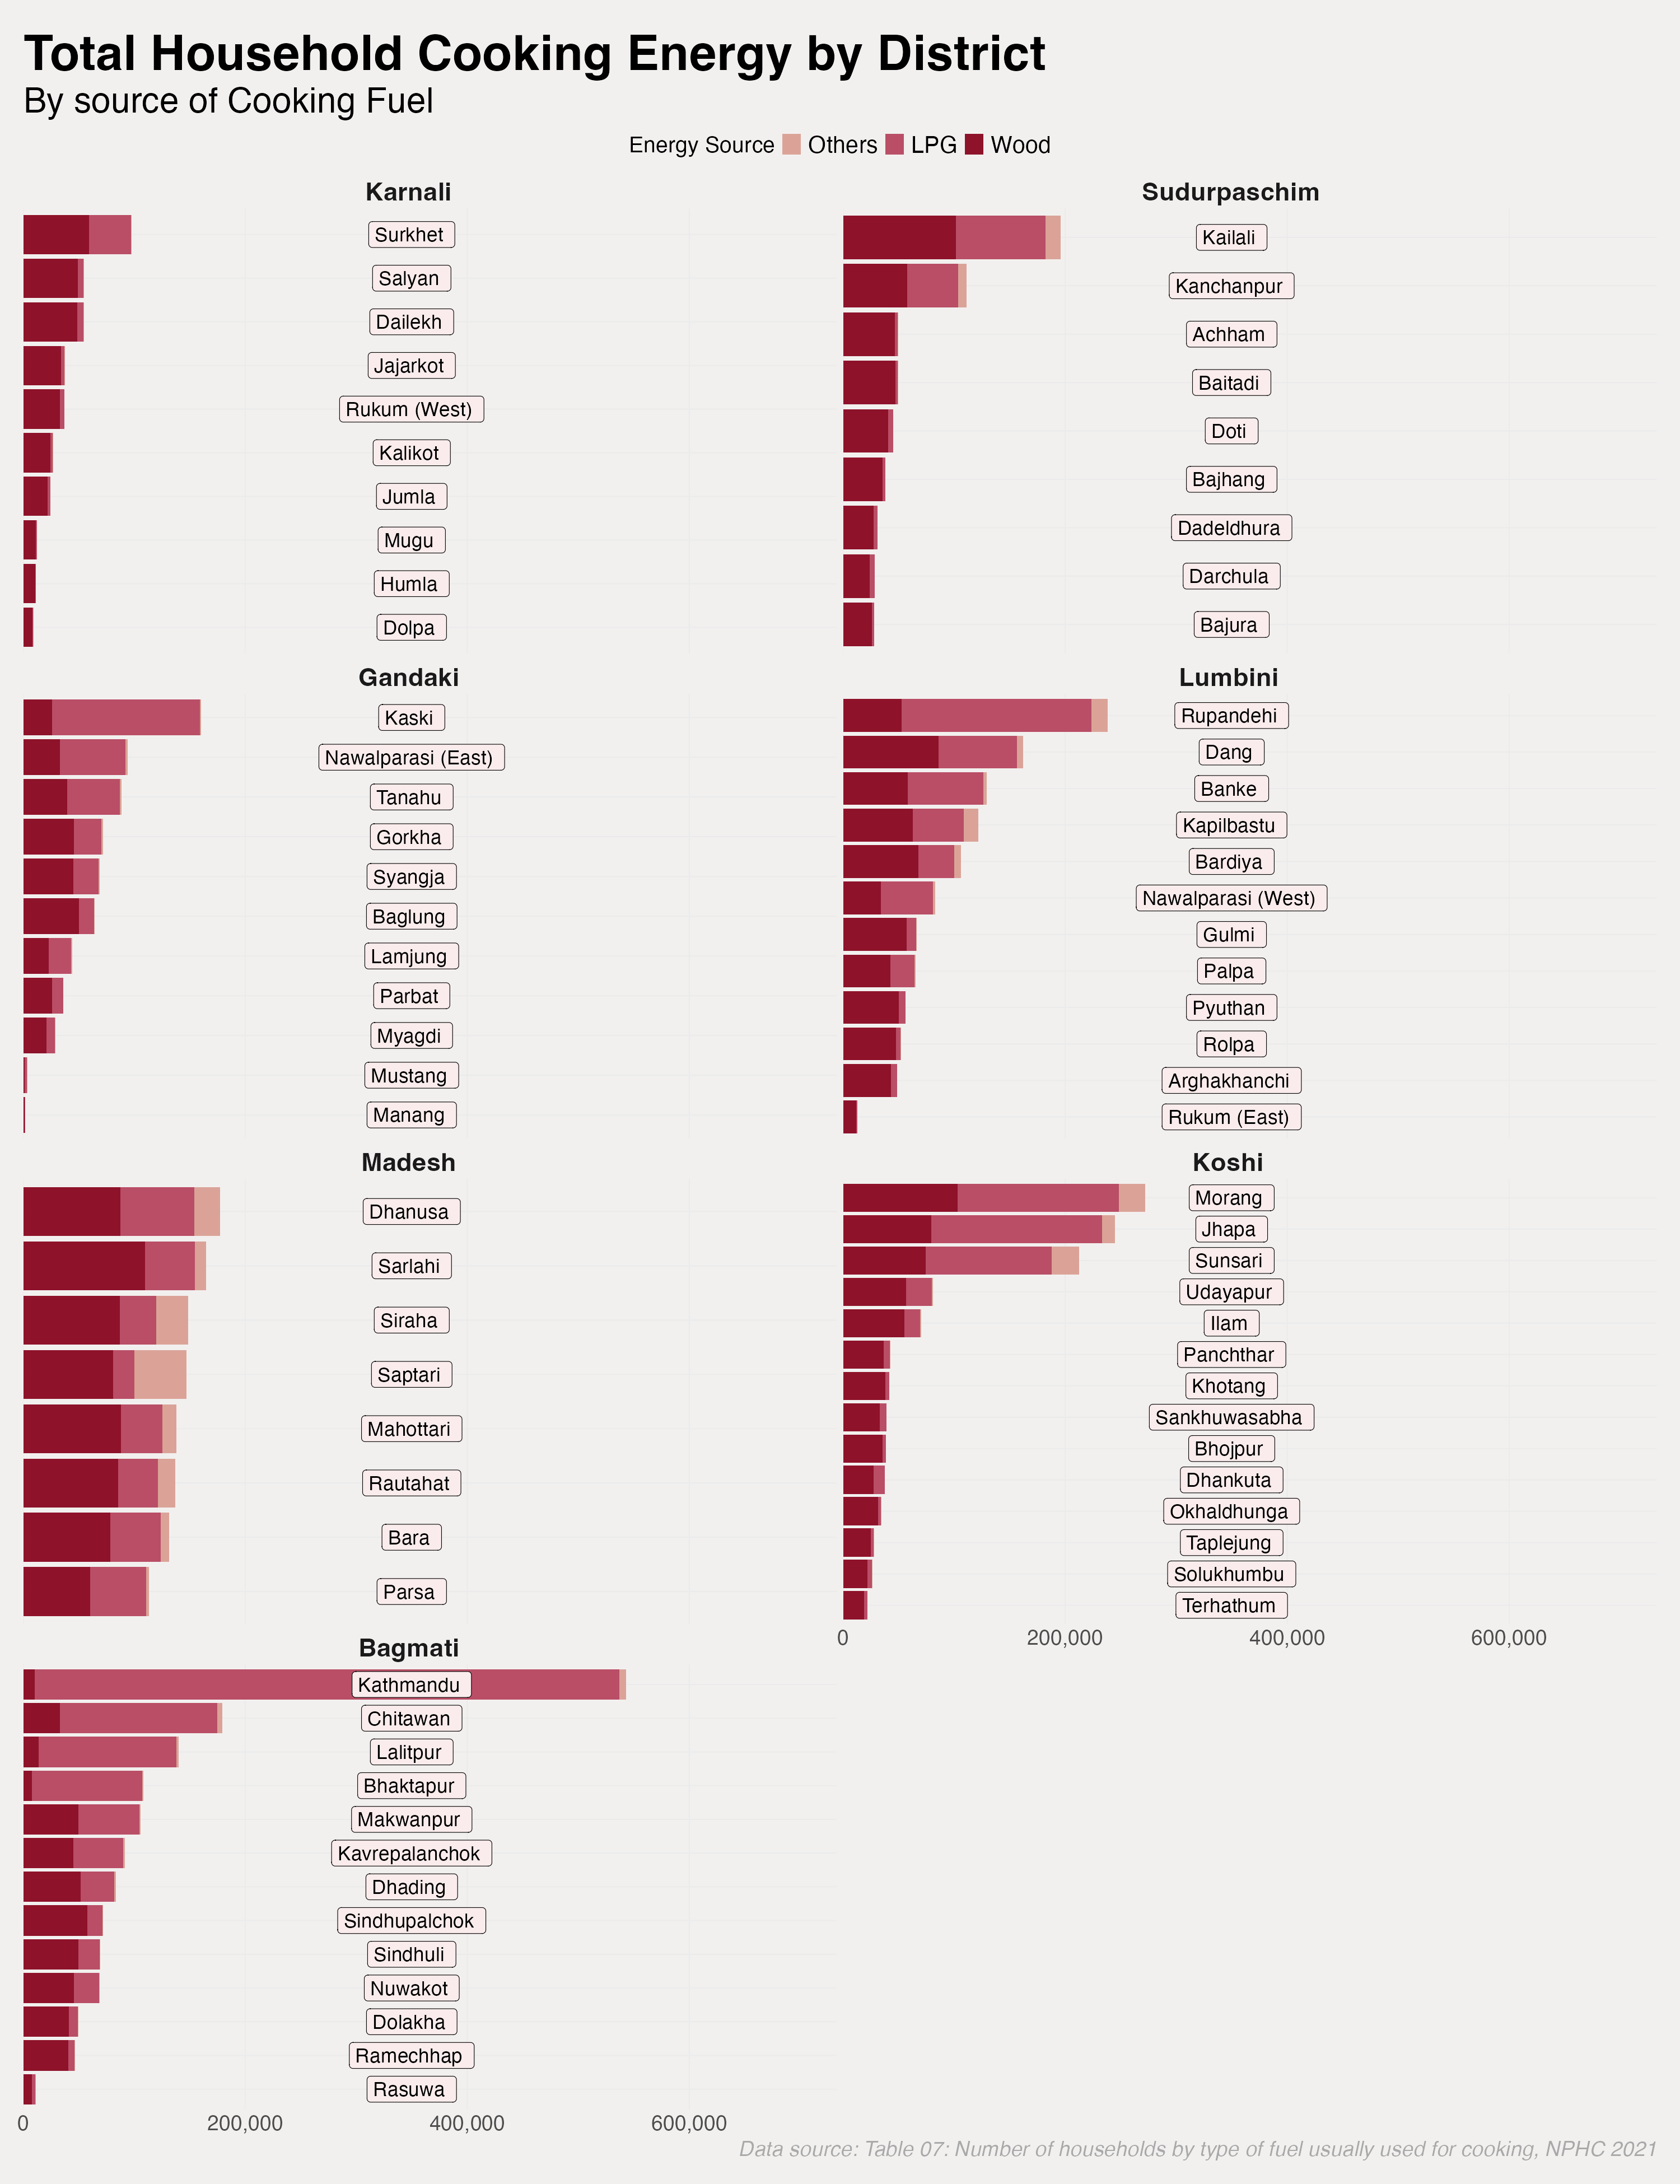
\includegraphics[keepaspectratio]{stacked_districts.png}}

}

\caption{\label{fig-stackeddist}Cooking Energy by District}

\end{figure}%




\end{document}
